\documentclass[aspectratio=169,xcolor=dvipsnames]{beamer}
\usetheme{SimplePlus}

% Math
\usepackage{nicefrac}

% Tipography stuff
\usepackage{booktabs} % Allows the use of \toprule, \midrule and \bottomrule in tables
\usepackage[english]{babel}
\usepackage{csquotes}
\usepackage{microtype}
\usepackage{pdfpages}
\usepackage{fontawesome5}
\usepackage{soul}
\usepackage{euler}
\usepackage{algorithm2e}
\usepackage{animate}
\usepackage{ifthen}

% Bibliography
\usepackage[giveninits,style=authoryear-comp,backend=biber]{biblatex}
\addbibresource{../fracbiblio.bib}
\newcommand\unnumbered{\setbeamertemplate{footline}{}}%\addtocounter{framenumber}{-1}
\renewcommand*{\bibfont}{\normalfont\small}

% Figures
\usepackage{tikz,pgfplots}
\usetikzlibrary{calc,arrows,patterns,matrix,external}
\usepackage{subfig}
\usepackage{graphicx} % Allows including images
\usepackage[american]{circuitikz}
\usepackage{tikz-network}
\tikzexternalize[prefix=Figures/] % activate and define figures/ as cache folder

% Links
\usepackage{hyperref}
\hypersetup{colorlinks,linkcolor=,urlcolor=MidnightBlue}

% Code
\usepackage{minted}

% Block matrices
\newcommand{\bigzero}{\mbox{\normalfont\Large\bfseries 0}}
\newcommand{\rvline}{\hspace*{-\arraycolsep}\vline\hspace*{-\arraycolsep}}
\newcommand{\R}{\mathbb{R}}
\newcommand{\bone}{{\bf 1}}
\newcommand{\evec}{{\bf e}}
\newcommand{\dvec}{{\bf d}}
\newcommand{\xvec}{{\bf x}}
\newcommand{\yvec}{{\bf y}}
\newcommand{\qvec}{{\bf q}}
\newcommand{\svec}{{\bf s}}
\newcommand{\pvec}{{\bf p}}
\newcommand{\tvec}{{\bf t}}
\definecolor{Ao}{rgb}{0.0, 0.5, 0.0}


\author{Fabio Durastante}
\title{An introduction to fractional calculus}
\subtitle{Fundamental ideas and numerics}
\institute{Università di Pisa\\\href{mailto:fabio.durastante@unipi.it}{\faEnvelope\;fabio.durastante@unipi.it}\\\href{https://fdurastante.github.io}{\faFirefox\;fdurastante.github.io}}
\date{June, 2022}

\newcommand{\de}{{\rm d}}


\begin{document}

{\unnumbered
\begin{frame}[t,plain,noframenumbering]
\titlepage
\vspace{-4em}
\includegraphics[width=2cm]{frame.png}
\end{frame}
}

\section{Questions in Complex Networks}

\begin{frame}{Questions in Complex Networks}
\vspace{1em}

\begin{columns}
\begin{column}{0.5\columnwidth}
\centering

{\begin{onlyenv}<1-3>
\begin{tikzpicture}[scale=0.9]
\only<1>{\Vertices{karatesimplevertex.csv}}
\only<2>{\Vertices{karateclustervertex.csv}}
\only<3>{\Vertices{karatecentralityvertex.csv}}
\only<1-3>{\Edges{karatesimpleedges.csv}}
\end{tikzpicture}
\end{onlyenv}}%
{\begin{onlyenv}<4>
\begin{tikzpicture}[scale=0.9]
\only<4>{\Vertices[size=.4]{karateedgevertex.csv}}
\only<4>{\Edges{karatebetweennessedges.csv}}
\end{tikzpicture}
\end{onlyenv}}
\vfill

A \alert{complex network} is a graph with \textbf{non-trivial} topological features, neither a structured graph (lattices, Cayley graphs, \emph{etc.}) nor a \emph{completely} random graph.
\end{column}
\begin{column}{0.5\columnwidth}
We are interested in tasks in \textbf{exploratory data analysis}, that is analyzing the data to \alert{summarize their main characteristics}:
\begin{itemize}
    \item[\faObjectUngroup] Divide the nodes into groups that are in the same community (\alert<2>{clustering}),
    \item[\faStar] Find the ``most relevant'' nodes in the network (\alert<3>{centrality}), 
    \item[\faArrowsAltH] Find the ``most relevant'' edge in the network (\alert<4>{edge centrality})
    \item[\faBalanceScale] Individuation of motifs, computation of fluxes, maximum cuts, \emph{etc.}
\end{itemize}
\end{column}
\end{columns}
\end{frame}

\begin{frame}[fragile]{\faBookDead\; Notation}

\begin{block}<1->{Network}
A {\it network} $G = (V,E)$ is defined as a pair of sets:  a set $V = \{1,2,\ldots,n\}$ of {\it nodes} and  a set $E\subset V\times V$ of {\it edges} between them.
\end{block}

\begin{columns}[t]
\begin{column}{0.5\columnwidth}
\centering
\only<2>{
\begin{block}<2>{Directed/Undirected}
If $\forall\,(i,j)\in E$ then $(j,i)\in E$ the network is said to be \textit{undirected} is {\it directed} otherwise.
\end{block}
\medskip}

\begin{onlyenv}<2>
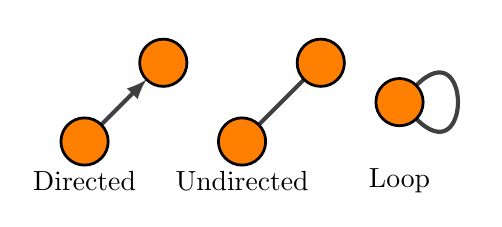
\begin{tikzpicture}
\Vertex[x=1,y=0,color=orange]{A}
\Vertex[x=2,y=1,color=orange]{B}
\Vertex[x=3,y=0,color=orange]{C}
\Vertex[x=4,y=1,color=orange]{D}
\Vertex[x=5,y=0.5,color=orange]{E}
\Edge[Direct=true](A)(B)
\Edge[Direct=false](C)(D)
\Edge(E)(E)
\Text[x=1,y=-0.5]{Directed}
\Text[x=3,y=-0.5]{Undirected}
\Text[x=5,y=-0.5]{Loop}
\end{tikzpicture}


An edge from a node to itself is called a {\it loop}. 
\end{onlyenv}
\begin{onlyenv}<3>
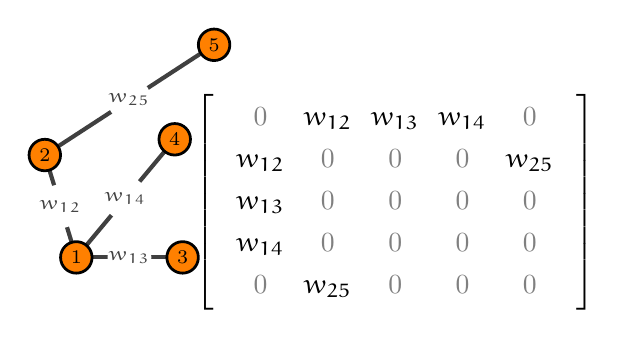
\begin{tikzpicture}
\Vertex[x=0.25,y=0,color=orange,size=.4,label=1]{A}
\Vertex[x=-0.15,y=1.3,color=orange,size=.4,label=2]{B}
\Vertex[x=1.6,y=0,color=orange,size=.4,label=3]{C}
\Vertex[x=1.50,y=1.5,color=orange,size=.4,label=4]{D}
\Vertex[x=2.,y=2.7,color=orange,size=.4,label=5]{E}
\Edge[label={w_{12}},Math=true](A)(B)
\Edge[label={w_{13}},Math=true](A)(C)
\Edge[label={w_{25}},Math=true](B)(E)
\Edge[label={w_{14}},Math=true](D)(A)
 \matrix[matrix of nodes, column sep = 0.01cm, row sep = 0.02cm, ,left delimiter={[},right delimiter={]}] at (4.3,0.7) {
 \textcolor{gray}{0} & $w_{12}$ & $w_{13}$ & $w_{14}$ & \textcolor{gray}{0} \\
 $w_{12}$ & \textcolor{gray}{0} & \textcolor{gray}{0} & \textcolor{gray}{0} & $w_{25}$ \\
 $w_{13}$ & \textcolor{gray}{0} & \textcolor{gray}{0} & \textcolor{gray}{0} & \textcolor{gray}{0} \\
 $w_{14}$ & \textcolor{gray}{0} & \textcolor{gray}{0} & \textcolor{gray}{0} & \textcolor{gray}{0} \\
 \textcolor{gray}{0} & $w_{25}$ & \textcolor{gray}{0} & \textcolor{gray}{0} & \textcolor{gray}{0} \\
 };
\end{tikzpicture}
\end{onlyenv}

\end{column}
\begin{column}{0.5\columnwidth}
\begin{block}<3>{Adjacency Matrix}
We represent a Network via its \alert{\it adjacency matrix} $A = (a_{ij})\in\mathbb{R}^{n\times n}$, entrywise defined as
	\[
	a_{ij} = 
	\begin{cases}
	w_{ij} & \text{if }(i,j)\in E \\
	0 & \text{otherwise}
	\end{cases}
	\]
    where $w_{ij}>0$ is the weight of edge $(i,j)$. 
\end{block}
\end{column}
\end{columns}

\end{frame}

\begin{frame}[fragile]{\faStar\; Centrality Measures: the limiting cases}
\begin{columns}
\begin{column}{0.5\columnwidth}
\begin{itemize}
\item \textbf{Degree centrality:} \[ d_i= \sum_{j=1}^n a_{ij} = (A\bone)_i\]
\item \textbf{Eigenvector centrality:} $\rho(A)>0$ the spectral radius of the irreducible $A\geq 0$ \[ x_i = \frac{1}{\rho(A)}\sum_{j=1}^n a_{ij} x_j\]
\end{itemize}
\end{column}
\begin{column}{0.5\columnwidth}
\centering
\begin{tikzpicture}[scale=0.8]
\only<1>{\Vertices{karateeigenvertex.csv}}
\only<2>{\Vertices{karatedegreevertex.csv}}
\Edges[lw=1]{karatesimpleedges.csv}
\end{tikzpicture}

\only<1>{\textbf{Degree centrality} is oblivious to the whole topology of the network.}

\only<2>{\textbf{Eigenvector centrality} considers both the number of neighbors and their importance when assigning scores to nodes.
}
\end{column}
\end{columns}
\end{frame}

\begin{frame}{\faWalking\; Walk based centralities and Matrix Functions}
\vspace{1em}
\begin{columns}
\begin{column}{0.5\columnwidth}
Consider the \textbf{analytic function} $f$ in $\{ z \in \mathbb{C}\,:\; |z| < R_f\}$:
\[f(z) = \sum_{r=0}^\infty c_r z^r, \qquad c_r\geq 0\] 
then \alert{under suitable hypothesis} on the spectrum of $A$ we can write: 
\[f(A) = \sum_{r=0}^\infty c_r A^r.\]
\alert{\faWalking} $(A^r)_{i_1,i_{r+1}}$ is the number of walks from $i_{1}$ to $i_{r+1}$.
\end{column}
\begin{column}{0.5\columnwidth}
\centering
\begin{onlyenv}<1>

{\begin{tikzpicture}[scale=0.8]
\Vertices{karatepathvertex.csv}
\Edges{karatepathssedges.csv}
\end{tikzpicture}}

A \alert{\it walk} of length $r$ is a sequence of $r+1$ nodes $i_1, i_2,\ldots, i_{r+1}$ such that $(i_\ell,i_{\ell+1})\in E$ for all $\ell = 1,\ldots,r$.
\end{onlyenv}

\begin{onlyenv}<2>
\begin{itemize}
    \item $(f(A))_{ij}$ is a \textbf{weighted sum} of the number of \textbf{all walks} of any length that start from node $i$ and end at node $j$,
    \item $c_r\to 0$ as $r$ increases thus \textbf{walks of longer lengths} are considered to be \textbf{less important},
    \item The \alert{most popular functions} used in networks science are $f(z) = e^z$ and $f(z) = (1+z)^{-1}$.
\end{itemize}
\end{onlyenv}
\end{column}
\end{columns}
\end{frame}



\begin{frame}[fragile]{\faWalking\; Walk based centralities}

\begin{columns}
\begin{column}{0.5\columnwidth}
\begin{itemize}
    \item \textbf{Subgraph centrality:}
    \[ 	s_i(f) = \evec_i^T f(A)\evec_i = \sum_{r=0}^\infty c_r (A^r)_{ii}. \]
    \item \textbf{Total} (node) \textbf{communicability:}
    \[ t_i(f) = \sum_{j=1}^n (f(A))_{ij} = \sum_{j=1}^n\sum_{r=0}^\infty c_r(A^r)_{ij} \]
\end{itemize}
\end{column}
\begin{column}{0.5\columnwidth}
\centering
\begin{tikzpicture}[scale=0.8]
\only<1>{\Vertices{karateexpertex.csv}}
\only<2>{\Vertices{karatetexpertex.csv}}
\Edges[lw=1]{karatesimpleedges.csv}
\end{tikzpicture}

\only<1>{\textbf{Subgraph centrality} accounts for the \alert{returnability of information} from a node to itself: it is a weighted count of all the subgraphs node $i$ is involved in.}

\only<2>{For the \textbf{total comunicability} the importance of a node depends on \alert{how well it communicates with the whole network}, itself included}

\end{column}
\end{columns}

\end{frame}

\section{Mittag-Leffler based centralities}

\begin{frame}{The Mittag-Leffler Function}
The {\it Mittag--Leffler  (ML) function}  is an analytic functions given, $\forall \alpha,\beta>0$, by
\begin{columns}
\begin{column}{0.5\columnwidth}
\[	E_{\alpha,\beta}(z) = \sum_{r=0}^\infty c_r(\alpha,\beta) z^r= \sum_{r=0}^{\infty} \frac{z^r}{\Gamma(\alpha r + \beta)}, \]
where 
\begin{itemize}
	\item $c_r(\alpha,\beta)=\Gamma(\alpha r + \beta)^{-1}$,
	\item $\Gamma(z)$ is the {\it Euler Gamma function}:
	$$
	\Gamma(z) = \int_{0}^{\infty}t^{z-1}e^{-t}dt.
	$$
\end{itemize}
For particular choices of $\alpha,\beta>0$, the ML function $E_{\alpha,\beta}(z)$ has a nice closed form descriptions.
\end{column}
\begin{column}{0.5\columnwidth}
\scriptsize
\centering

\begin{tabular}{ccl}
	\toprule
	$\alpha$ & $\beta$ & Function \\
	\midrule
	0 & 1 & $(1-z)^{-1}$ \\ & & \alert{Resolvent} \\
	1 & 1 & $\exp(z)$ \\ & & \alert{Exponential} \\
	$\frac{1}{2}$ & 1 & $\exp(z^2)\operatorname{erfc}(-z)$ \\ & & Error Function\footnotemark \\
	2 & 1 & $\cosh(\sqrt{z})$ \\ & & Hyperbolic Cosine \\
	2 & 2 & $\sinh(\sqrt{z})/\sqrt{z}$ \\ & & Hyperbolic Sine \\
	%3 & 1 & $1/3 [\exp(z^{1/3})+\ldots$  & \\
	%& & $\;\ldots 2 \exp(-{z^{1/3}}/{2}) \cos(\sqrt{3} z^{1/3}/2)]$ \\
	4 & 1 & $\frac{1}{2} [\cos(z^{1/4}) + \cosh(z^{1/4})]$ \\
	%\multirow{2}{*}{ 1 } & \multirow{2}{*}{$r= 2,3,\ldots$} & \multirow{2}{*}{$z^{1-r}(e^z - \sum_{k=0}^{r-2} \frac{z^k}{k!})$} & Shifted exponential: \\& &  & $\varphi_{r-1}(z) = \sum_{k=0}^\infty \frac{z^k}{(k+r-1)!}$ \\ 
	1 & $k\geq2$ &$z^{1-k}(e^z - \sum_{r=0}^{k-2} \frac{z^r}{r!})$ \\ & & $\varphi_{k-1}(z) = \sum_{r=0}^\infty \frac{z^r}{(r+k-1)!}$ \\
	\bottomrule
\end{tabular}
\end{column}
\end{columns}
\end{frame}

\begin{frame}{The Mittag-Leffler Function: other occurrences}
Another use of it is in the case $E_{1,2}(z) = \psi_1(z)$ for computing the \textbf{non-backtracking exponential generating function} for simple graphs~\parencite{MR3842589} is:
\[
\sum_{r=0}^\infty \frac{p_r(A)}{r!} = 
\begin{bmatrix} I & 0\end{bmatrix} \psi_1(Y) 
\begin{bmatrix} A \\A^2-D\end{bmatrix} + I,
\]
where $p_r(A)$ is a matrix whose entries represent the \alert{number of non-backtracking walks of length $r$ between any two given nodes}
\begin{onlyenv}<1>
\begin{columns}
\begin{column}{0.4\columnwidth}
\begin{onlyenv}<1>
\begin{center}
\begin{tikzpicture}[scale=0.45]
\Vertices{mycielskian4.csv}
\Edges{mycielskian4edge.csv}
\end{tikzpicture}
\end{center}
\end{onlyenv}
\end{column}
\begin{column}{0.6\columnwidth}
\begin{block}{Backtracking walk}
A walk is \emph{backtracking} if it contains at least one pair of successive edeges of the form $i \mapsto j$, $j\mapsto i$. We say that
is \emph{non-backtracking} otherwise.
\end{block}
\end{column}
\end{columns}
\end{onlyenv}
\begin{onlyenv}<2-3>
\begin{columns}
\begin{column}{0.5\columnwidth}
\only<2>{\centering 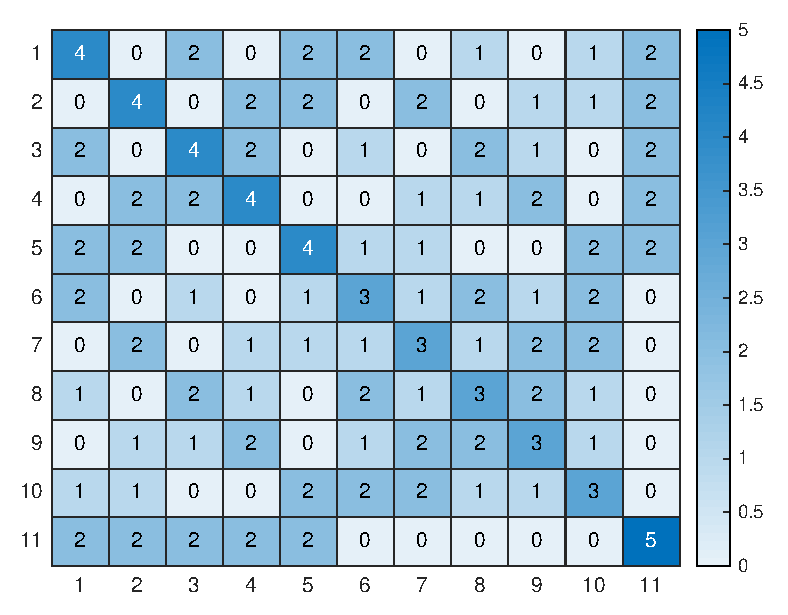
\includegraphics[width=0.5\columnwidth]{back2.eps}\\ $A^2$}%
\only<3>{\centering 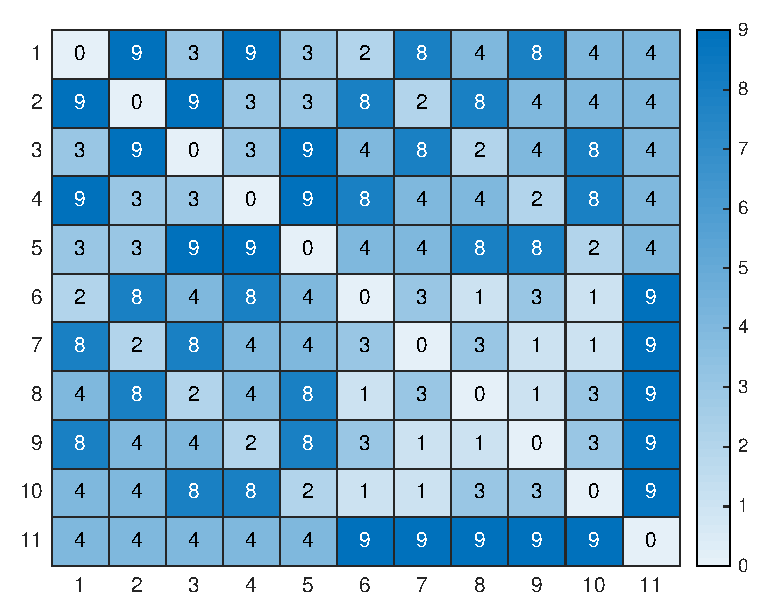
\includegraphics[width=0.5\columnwidth]{back3.eps}\\ $A^3$}%
\end{column}
\begin{column}{0.5\columnwidth}
\only<2>{\centering 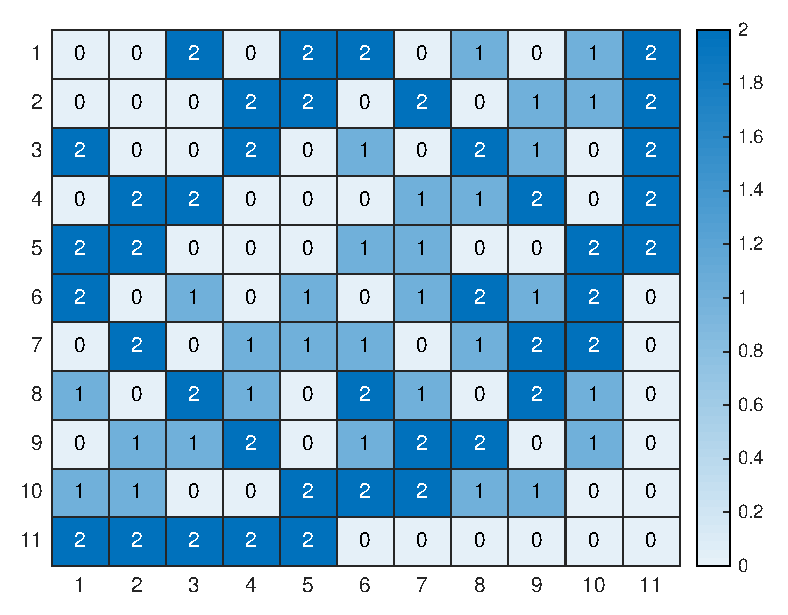
\includegraphics[width=0.5\columnwidth]{nonback2.eps}\\ $p_2(A)$}%
\only<3>{\centering 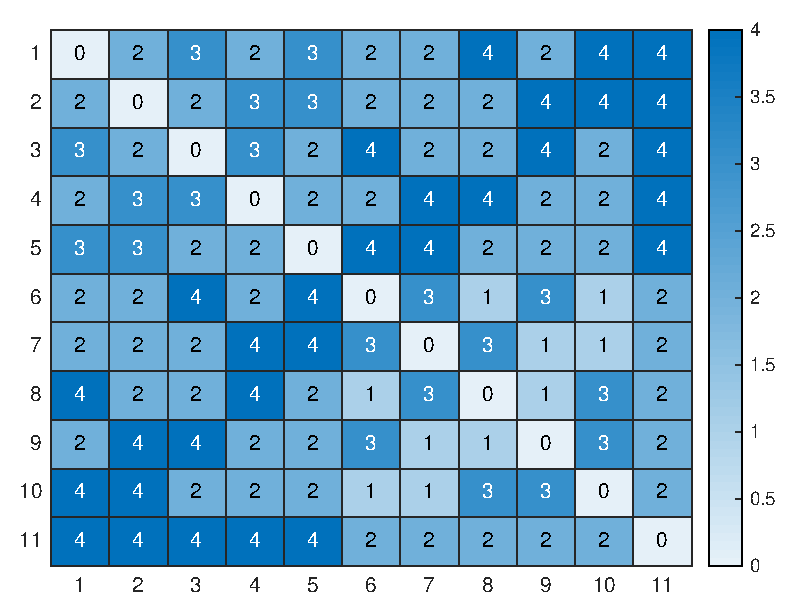
\includegraphics[width=0.5\columnwidth]{nonback3.eps}\\ $p_3(A)$}%
\end{column}
\end{columns}
\end{onlyenv}
\only<4>{$D = \operatorname{diag}(A)$, and $Y$ is the first companion linearization of the matrix polynomial $(D-I) -A\lambda +I\lambda^2$:
\[
Y = 
\begin{bmatrix}
0 & I \\
I-D & A
\end{bmatrix}
.\]}
\end{frame}

\begin{frame}{The Mittag-Leffler Function: other occurrences}

To compute \textbf{centrality} and \textbf{communicability} indices for \textbf{directed networks}, if $A$ is the \alert{adjacency matrix of a directed graph}, then
\[
\mathcal{A} = \begin{bmatrix}
O & A \\
A^T & O
\end{bmatrix} \; \Rightarrow \only<1>{\; \exp(\mathcal{A}) = \begin{bmatrix}
\cosh(\sqrt{AA^T}) & A(\sqrt{A^TA})^\dagger\sinh(\sqrt{A^TA}) \\
\sinh(\sqrt{A^TA})(\sqrt{A^TA})^\dagger A^T & \cosh(\sqrt{A^TA})) 
\end{bmatrix}}\only<2->{
\; \exp(\mathcal{A}) = \begin{bmatrix}
E_2(AA^T) & A E_{2,2}(A^TA)\\
E_{2,2}(A^TA) A & E_2(A^TA) 
\end{bmatrix}
}
\]
\begin{columns}
\begin{column}{0.4\columnwidth}
Centrality and communicability indices for \alert<1>{directed networks} defined
by exploiting the representation of such networks as \alert{bipartite graphs}; details in~\parencite{MR3005305}.
\end{column}
\begin{column}{0.6\columnwidth}
\begin{onlyenv}<1>
\begin{center}
\begin{tikzpicture}[scale=0.65]
\Vertices{GD01_b.csv}
\Edges{GD01_bedge.csv}
\end{tikzpicture}
\end{center}
\end{onlyenv}
\begin{onlyenv}<2->
\begin{center}
\begin{tikzpicture}[scale=0.6]
\Vertices{GD01_b_bip.csv}
\Edges{GD01_bedge_bip.csv}
\end{tikzpicture}
\end{center}
\end{onlyenv}
\end{column}
\end{columns}

\end{frame}


\begin{frame}{\faLightbulb\; Defining Mittag-Leffler based centralities}
\begin{columns}
\begin{column}{0.5\columnwidth}
\centering
	
For each choice of $\alpha,\beta>0$ we want to define \faWalking\, centralities based on
	\begin{equation*}
	\begin{split}
		E_{\alpha,\beta}(z) = & \;\sum_{r=0}^\infty c_r(\alpha,\beta) z^r \\ = & \; \sum_{r=0}^{\infty} \frac{z^r}{\Gamma(\alpha r + \beta)},
	\end{split}
	\end{equation*}	
	
	
The idea of a \faWalking\, centrality relies on the fact that walks of longer lengths  are less important, \alert{\textbf{but}} $c(r):=\Gamma(\alpha r+1)$ is not monotonic for certain values of $\alpha\in(0,1)$!

\end{column}
\begin{column}{0.5\columnwidth}
\centering
% This file was created by matlab2tikz.
%
%The latest updates can be retrieved from
%  http://www.mathworks.com/matlabcentral/fileexchange/22022-matlab2tikz-matlab2tikz
%where you can also make suggestions and rate matlab2tikz.
%
\definecolor{mycolor1}{rgb}{0.00000,0.44700,0.74100}%
\definecolor{mycolor2}{rgb}{0.85000,0.32500,0.09800}%
\definecolor{mycolor3}{rgb}{0.92900,0.69400,0.12500}%
\definecolor{mycolor4}{rgb}{0.49400,0.18400,0.55600}%
\definecolor{mycolor5}{rgb}{0.46600,0.67400,0.18800}%
\definecolor{mycolor6}{rgb}{0.30100,0.74500,0.93300}%
\definecolor{mycolor7}{rgb}{0.63500,0.07800,0.18400}%
%
\begin{tikzpicture}

\begin{axis}[%
width=0.7\columnwidth,
height=2.3in,
at={(1.29in,0.481in)},
scale only axis,
xmin=0,
xmax=3,
xlabel style={font=\color{white!15!black}},
xlabel={r},
ymin=0,
ymax=1.2,
ylabel style={font=\color{white!15!black}},
ylabel={$\Gamma\text{(}\alpha\text{ r + 1)}^{\text{-1}}$},
axis background/.style={fill=white},
axis x line*=bottom,
axis y line*=left,
legend columns=3,
legend style={at={(0.03,0.03)}, anchor=south west, legend cell align=left, align=left, draw=white!15!black, font=\footnotesize}
]
\addplot [color=mycolor1, line width=2.0pt, mark=o, mark options={solid, mycolor1}]
  table[row sep=crcr]{%
0	1\\
1	1\\
2	1\\
3	1\\
};
\addlegendentry{$\alpha\text{ = 0.0}$}

\addplot [color=mycolor2, dashed, line width=2.0pt, mark=+, mark options={solid, mycolor2}]
  table[row sep=crcr]{%
0	1\\
1	1.05113700611178\\
2	1.08912442105834\\
3	1.1142425085473\\
};
\addlegendentry{$\alpha\text{ = 0.1}$}

\addplot [color=mycolor3, dotted, line width=2.0pt, mark=asterisk, mark options={solid, mycolor3}]
  table[row sep=crcr]{%
0	1\\
1	1.08912442105834\\
2	1.12706049798603\\
3	1.11917495407012\\
};
\addlegendentry{$\alpha\text{ = 0.2}$}

\addplot [color=mycolor4, dashdotted, line width=2.0pt, mark=*, mark options={solid, mycolor4}]
  table[row sep=crcr]{%
0	1\\
1	1.1142425085473\\
2	1.11917495407012\\
3	1.03975413434764\\
};
\addlegendentry{$\alpha\text{ = 0.3}$}

\addplot [color=mycolor5, line width=2.0pt, mark=x, mark options={solid, mycolor5}]
  table[row sep=crcr]{%
0	1\\
1	1.12706049798603\\
2	1.07367127403083\\
3	0.90760368421528\\
};
\addlegendentry{$\alpha\text{ = 0.4}$}

\addplot [color=mycolor6, dashed, line width=2.0pt, mark=triangle, mark options={solid, rotate=270, mycolor6}]
  table[row sep=crcr]{%
0	1\\
1	1.12837916709551\\
2	1\\
3	0.752252778063675\\
};
\addlegendentry{$\alpha\text{ = 0.5}$}

\addplot [color=mycolor7, dotted, line width=2.0pt, mark=triangle, mark options={solid, mycolor7}]
  table[row sep=crcr]{%
0	1\\
1	1.11917495407012\\
2	0.90760368421528\\
3	0.596484041128241\\
};
\addlegendentry{$\alpha\text{ = 0.6}$}

\addplot [color=mycolor1, dashdotted, line width=2.0pt, mark=square, mark options={solid, mycolor1}]
  table[row sep=crcr]{%
0	1\\
1	1.10054740552367\\
2	0.805043212847163\\
3	0.455037664983454\\
};
\addlegendentry{$\alpha\text{ = 0.7}$}

\addplot [color=mycolor2, line width=2.0pt, mark=diamond, mark options={solid, mycolor2}]
  table[row sep=crcr]{%
0	1\\
1	1.07367127403083\\
2	0.699484346293826\\
3	0.335434672019651\\
};
\addlegendentry{$\alpha\text{ = 0.8}$}

\addplot [color=mycolor3, dashed, line width=2.0pt, mark=star, mark options={solid, mycolor3}]
  table[row sep=crcr]{%
0	1\\
1	1.03975413434764\\
2	0.596484041128241\\
3	0.239770676584677\\
};
\addlegendentry{$\alpha\text{ = 0.9}$}

\addplot [color=mycolor4, dotted, line width=2.0pt, mark=star, mark options={solid, mycolor4}]
  table[row sep=crcr]{%
0	1\\
1	1\\
2	0.5\\
3	0.166666666666667\\
};
\addlegendentry{$\alpha\text{ = 1.0}$}

\end{axis}
\end{tikzpicture}%

\end{column}
\end{columns}
\end{frame}

\begin{frame}{\faHammer\; Enforcing monotonicity}

\begin{alertblock}{Lemma (Arrigo, D.)}
Suppose that $\alpha \in (0,1)$. The coefficients $\widetilde{c}_r(\alpha,\gamma) = \gamma^r c_r(\alpha)$ defining the power series for the entire function $\widetilde{E}_\alpha(z) = E_{\alpha}(\gamma z)$ are monotonically decreasing as a function of $r = 0,1,2,\ldots$ for all $0<\gamma<\Gamma(\alpha+1)$.
\end{alertblock}

\textbf{Proof.} \only<1>{For each $\alpha\in(0,1)$ we want to determine conditions on $\gamma = \gamma(\alpha)$ that imply that 
    \[\Tilde{c}_r(\alpha,\gamma) \geq \Tilde{c}_{r+1}(\alpha,\gamma) \quad \text{for all } r\in\mathbb{N} \]
    From the definition of $\Tilde{c}_r(\alpha,\gamma)$ we have that the above inequality is equivalent to verifying 
    \begin{equation*}
    \gamma \leq \frac{\Gamma (\alpha r+\alpha+1)}{\Gamma (\alpha r+1)}, \quad \text{for all } r\geq 0 
    \end{equation*}
    since $\gamma>0$ and $\Gamma(x)>0$ for all $x\geq 0$.} \only<2->{
	Since    $H_x$, the \emph{Harmonic number} for $x\in\mathbb{R}$, is an increasing function of $x$, $\alpha>0$ by hypothesis, and $\Gamma(x)>0$ for all $x\geq 0$, it follows that 
\[    \frac{d}{dx}\left(\frac{\Gamma (\alpha x+\alpha+1)}{\Gamma (\alpha x+1)}\right)  = \frac{\alpha \left(H_{ \alpha(x+1)}-H_{\alpha x}\right) \Gamma (\alpha x+\alpha+1)}{\Gamma (\alpha x+1)}\geq 0,\]
and thus the minimum of $\frac{\Gamma (\alpha x+\alpha+1)}{\Gamma (\alpha x+1)}$ is achieved at $x=0$.    
    }
\begin{onlyenv}<3>\vspace{-0.5em}
\begin{exampleblock}{\faLuggageCart\;Take-home message}
\small Mittag--Leffler functions with $\alpha\in (0,1)$ can be employed since they have a power series expansion that can be interpreted in terms of walks; however, care should be taken since to enforce monotonic behavior of the coefficients.
\end{exampleblock}
\end{onlyenv}
\end{frame}

\begin{frame}{\faEye\; A matter of magnitude}
\only<1>{Adjacency matrices of simple graphs have \alert{\textbf{positive}} and \textbf{negative} eigenvalues ($\operatorname{tr}(A) = 0$)!}\only<2>{We know asymptotic expansions for the ML function for $\theta \in (\frac{\pi \alpha}{2},\min(\pi,\alpha\pi))$ and any $p \in \mathbb{N}$:}\only<1>{\medskip}
\begin{onlyenv}<1>	
\begin{columns}
\begin{column}{0.5\columnwidth}
\centering
\begin{tikzpicture}[scale=0.75]
\Vertices{dolphinssimplevertex.csv}
\Edges{dolphinssimpleedges.csv}
\end{tikzpicture}

Newmann/Dolphins
\end{column}
\begin{column}{0.5\columnwidth}
\centering
% This file was created by matlab2tikz.
%
%The latest updates can be retrieved from
%  http://www.mathworks.com/matlabcentral/fileexchange/22022-matlab2tikz-matlab2tikz
%where you can also make suggestions and rate matlab2tikz.
%
\definecolor{mycolor1}{rgb}{0.00000,0.44700,0.74100}%
%
\begin{tikzpicture}

\begin{axis}[%
width=0.8\columnwidth,
height=1.3in,
at={(0.758in,0.481in)},
scale only axis,
xmin=0,
xmax=63,
xlabel style={font=\color{white!15!black}},
xlabel={i},
ymin=-4,
ymax=9,
ytick={-4,0,5,8},
ylabel style={font=\color{white!15!black}},
ylabel={$\lambda{}_\text{i}$},
axis background/.style={fill=white},
legend style={legend cell align=left, align=left, draw=white!15!black}
]
\addplot [color=mycolor1, draw=none, mark=o, mark options={solid, mycolor1}]
  table[row sep=crcr]{%
1	-3.82102838716202\\
2	-3.72415819432181\\
3	-3.4357406031923\\
4	-3.20495883651448\\
5	-2.9846680162525\\
6	-2.77091116129579\\
7	-2.67924086940963\\
8	-2.60934155633283\\
9	-2.45041047792569\\
10	-2.3094514462268\\
11	-2.14496218193445\\
12	-2.07830114995129\\
13	-2.0014330573532\\
14	-1.86086556274021\\
15	-1.75466625249464\\
16	-1.62336128432302\\
17	-1.60806582663979\\
18	-1.43508682799281\\
19	-1.31253117208902\\
20	-1.12711186146586\\
21	-1.01228758663734\\
22	-0.979841067177472\\
23	-0.83937695316594\\
24	-0.803709803923248\\
25	-0.683740375935387\\
26	-0.597066689576083\\
27	-0.502117205533115\\
28	-0.40265383662247\\
29	-0.316948368195531\\
30	-0.244840375983323\\
31	-0.177854253204695\\
32	-0.0154595975443203\\
33	-1.41272710568174e-15\\
34	1.1058156362822e-15\\
35	0.0320169756041258\\
36	0.144617131798515\\
37	0.154500109833371\\
38	0.213449909831518\\
39	0.317176968768388\\
40	0.432403750943383\\
41	0.448215460603506\\
42	0.729132998998056\\
43	0.768831406187273\\
44	0.880331511235151\\
45	1.0070897889413\\
46	1.18561166306807\\
47	1.26808651586724\\
48	1.31348718185841\\
49	1.36573478457122\\
50	1.46429392876631\\
51	1.61915251269497\\
52	1.85057942716429\\
53	2.0071583132243\\
54	2.2886543549218\\
55	2.48118371951807\\
56	2.8895601740307\\
57	3.09582353812408\\
58	3.45684272627871\\
59	4.13797087490276\\
60	4.83036007923221\\
61	5.93631101677066\\
62	7.19361401537868\\
};
%\addlegendentry{data1}

\end{axis}
\end{tikzpicture}%

$E_{0.4,1}(\rho(A)) = E_{0.4,1}(7.1936\ldots) \approx \alert{10^{60}}$
\end{column}
\end{columns}
\end{onlyenv}
\begin{onlyenv}<2>

\begin{alertblock}{Proposition \parencite[Proposition~3.6]{MR3244285}}
Let $0<\alpha<2$ and $\theta \in (\frac{\pi \alpha}{2},\min(\pi,\alpha\pi))$. Then we have the following asymptotics for the Mittag--Leffler function for any~$p \in \mathbb{N}$
\begin{eqnarray*}
	E_{\alpha}(z) = \frac{1}{\alpha} e^{z^{\frac{1}{\alpha}}} - \sum_{k=1}^{p} \frac{z^{-k}}{\Gamma(1-\alpha k)} + O(\lvert z\rvert^{-1-p}), \, \lvert z \rvert \rightarrow + \infty, \, \lvert \arg(z)\rvert \leq \theta,\\
	E_{\alpha}(z) = - \sum_{k=1}^{p} \frac{z^{-k}}{\Gamma(1-\alpha k)} + O(\lvert z\rvert^{-1-p}), \, \lvert z \rvert \rightarrow + \infty, \, \theta \leq \lvert \arg(z)\rvert \leq \pi.\nonumber
\end{eqnarray*}
\end{alertblock}

\begin{center}
We need to set the $\gamma$ to \alert{\textbf{scale the largest modulus eigenvalue}} in the computable range!
\end{center}

\end{onlyenv}
\end{frame}

\begin{frame}{\faHammer\; A matter of magnitude}

\begin{block}{Lemma (Arrigo, D.)}
Suppose that $\alpha \in (0,1]$, and $A  \in \mathbb{R}^{n \times n}$ is symmetric. Then for all 
\[\gamma \leq \frac{1}{\lambda_{\max}(A)}\left(\bar{K}\log(10) + \log(\alpha)\right)^\alpha\]
it holds that $\max_{i,j}(|E_{\alpha}(\gamma A)|)_{i,j} \leq \Bar{N}$ where $\Bar{N} \approx 10^{\Bar{K}}$ for a given $\bar{K} \in \mathbb{N}$ is the largest representable number on a given machine.
\end{block}

\textbf{Proof.} We have $\lambda_{\max}(\gamma A) =\gamma \lambda_{\max}(A) \in \mathbb{R}$, since $A$ is symmetric; then empolying the asymptotic expansion, and using the fact that $\arg(z) = 0$ for $z \in \mathbb{R}$, for $p = 0$ we find   
	\begin{equation*}
	\frac{1}{\alpha} e^{(\gamma\lambda_{\max}(A))^{\frac{1}{\alpha}}} \leq \bar{N} \approx 10^{\bar{K}}, 
	\end{equation*}
    which immediately yields the conclusion.
\end{frame}

\begin{frame}{Well-posedness and machine representability}
\begin{columns}
	\begin{column}{0.5\columnwidth}
		\begin{block}{Subgraph and total communicability centralities}
				Let $A$ be the adjacency matrix of a simple graph $G = (V, E)$. Let $\alpha\in[0,1]$ and \alert{let $0<\gamma \leq \mu(\alpha)$}. 
				Then, for all nodes $i\in V = \{1,2,\ldots,n\}$ we define: 
				\begin{itemize}
					\item ML-subgraph centrality:\vspace*{-3pt} 
					\[s_i(\widetilde{E}_\alpha) = E_\alpha(\gamma A)_{ii}\]
					\item ML-total communicability:\vspace*{-3pt} 
					\[t_i(\widetilde{E}_\alpha) = (E_\alpha(\gamma A)\bone)_{i}\]
				\end{itemize}
		\end{block}
	\end{column}
	\begin{column}{0.5\columnwidth}
	\begin{block}{\small Proposition (Arrigo, D.)}
	\small
	Let $A$ be the adjacency matrix of an undirected network with at least one edge and let $\rho(A)>0$ be its spectral radius. Moreover, let $\Bar{N}\approx 10^{\Bar{K}}$ be the largest representable number on a given machine. Then the  Mittag--Leffler function $\widetilde{E}_\alpha(z) = E_{\alpha}(\gamma z)$ is representable in the machine, and admits a series expansion with decreasing coefficients when $\alpha \in (0,1)$ and $0< \gamma \leq  \mu(\alpha)$
	\begin{equation*}
	\alert{\mu(\alpha)}:=\min\begin{cases} \Gamma(\alpha+1),\\\displaystyle \frac{\left( \bar{K}\log(10) + \log(\alpha)\right)^\alpha}{\rho(A)}\end{cases}
	\end{equation*}
	\end{block}
	\end{column}
\end{columns}
\end{frame}

\begin{frame}{\faLightbulb\; The main idea behind ML centralities}\vspace{-0.7em}
\begin{columns}
\begin{column}{0.6\columnwidth}
\begin{block}{\small Theorem \parencite{MR3354998}}
		\small Let $G= (V,E)$ be a connected, undirected, unweighted network with primitive $A$, and $f$ an analytic function with strictly positive series expansion defined on the spectrum of~$A$.\vspace{-0.5em}
		\begin{itemize}
			\item For $\gamma \rightarrow 0^+$, the rankings produced by both $\svec(\gamma)$ and $\tvec(\gamma)$ converge to those produced by the vector of degree centralities,
			\item If in addition $f$ is analytic on the whole real axis or is such that,\vspace{-0.5em}
			\[ \sum_{r = 0}^{\infty} c_r R_f^r = \lim_{\gamma \rightarrow 1^-} \sum_{r=0}^{\infty} c_r t^r R_f^t = +\infty, \]
			then, for $t\rightarrow R_f/\rho(A)$, the rankings produced by both $\svec(\gamma)$ and $\tvec(\gamma)$ converge to those produced by the eigenvector 
			centrality.
		\end{itemize}
\end{block}
\end{column}
\begin{column}{0.4\columnwidth}
	\centering
	
	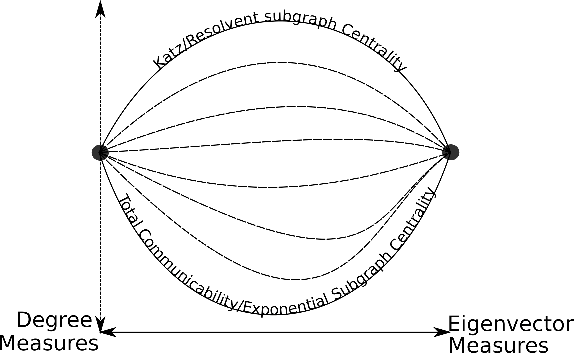
\includegraphics[width=\columnwidth]{asymptoticmagic.png}
	
	\vfill\textcolor{orange}{\faLightbulb} \small We build measures that ``interpolate asymptotically'' between four other ``central'' centralities measures:
	Degree, Eigenvector, Exponential and Resolvent walk centralities.
\end{column}
\end{columns}
\end{frame}

\begin{frame}{\faCalculator\; ML matrix-function vector products}
The tasks of computing \alert{ML-subgraph centrality} and \alert{ML-total communicability} relies on the task of computing the ML function ``with matrix argument'', which is a delicate task 
\begin{itemize}
	\item[\faFile] We can use, e.g., the techniques and the code developed in \parencite{MatrixML},
	\item[\faHandPointRight] then for ``large networks'' we adopt a polynomial Krylov subspace projection technique \parencite{MoretNovatiML} to handle the computations
	\begin{itemize}
		\only<1>{\item \normalsize For $V$ a basis of $\mathcal{K}_m(A,\mathbf{1}) = \operatorname{span}\{\mathbf{v},A\mathbf{v},\ldots,A^{m-1}\mathbf{v}\}$ 
		\[ \textbf{t}(\gamma) \approx V E_\alpha(\gamma V^T A V) V^T \mathbf{1},  \]}
		\item \normalsize For $V$ a basis of $\mathcal{K}_m(A,\mathbf{e}_i) = \operatorname{span}\{\mathbf{e}_i,A\mathbf{e}_i,\ldots,A^{m-1}\mathbf{e}_i\}$,
		\[ s_i(\gamma) \approx \mathbf{e}_{i}^T V E_\alpha(\gamma V^T A V) V^T\mathbf{e}_{i}.  \]
	\end{itemize}
\end{itemize}
\only<2>{\emph{Subgraph centrality} is computationally \textbf{quite expensive} to derive for all nodes \alert{but} approximation techniques for few top ranked nodes are available \parencite{MR3143833}.}
\end{frame}

\subsection{Numerical Examples}

\begin{frame}{Numerical Examples}
We compare \only<1>{subgraph centrality}\only<2>{total comunicability} with \textbf{eigenvector centrality} and \textbf{degree centrality} as we let $\alpha$ and $\gamma$ vary on a real-world network

\begin{columns}
\begin{column}{0.5\columnwidth}
\centering\footnotesize

\only<1>{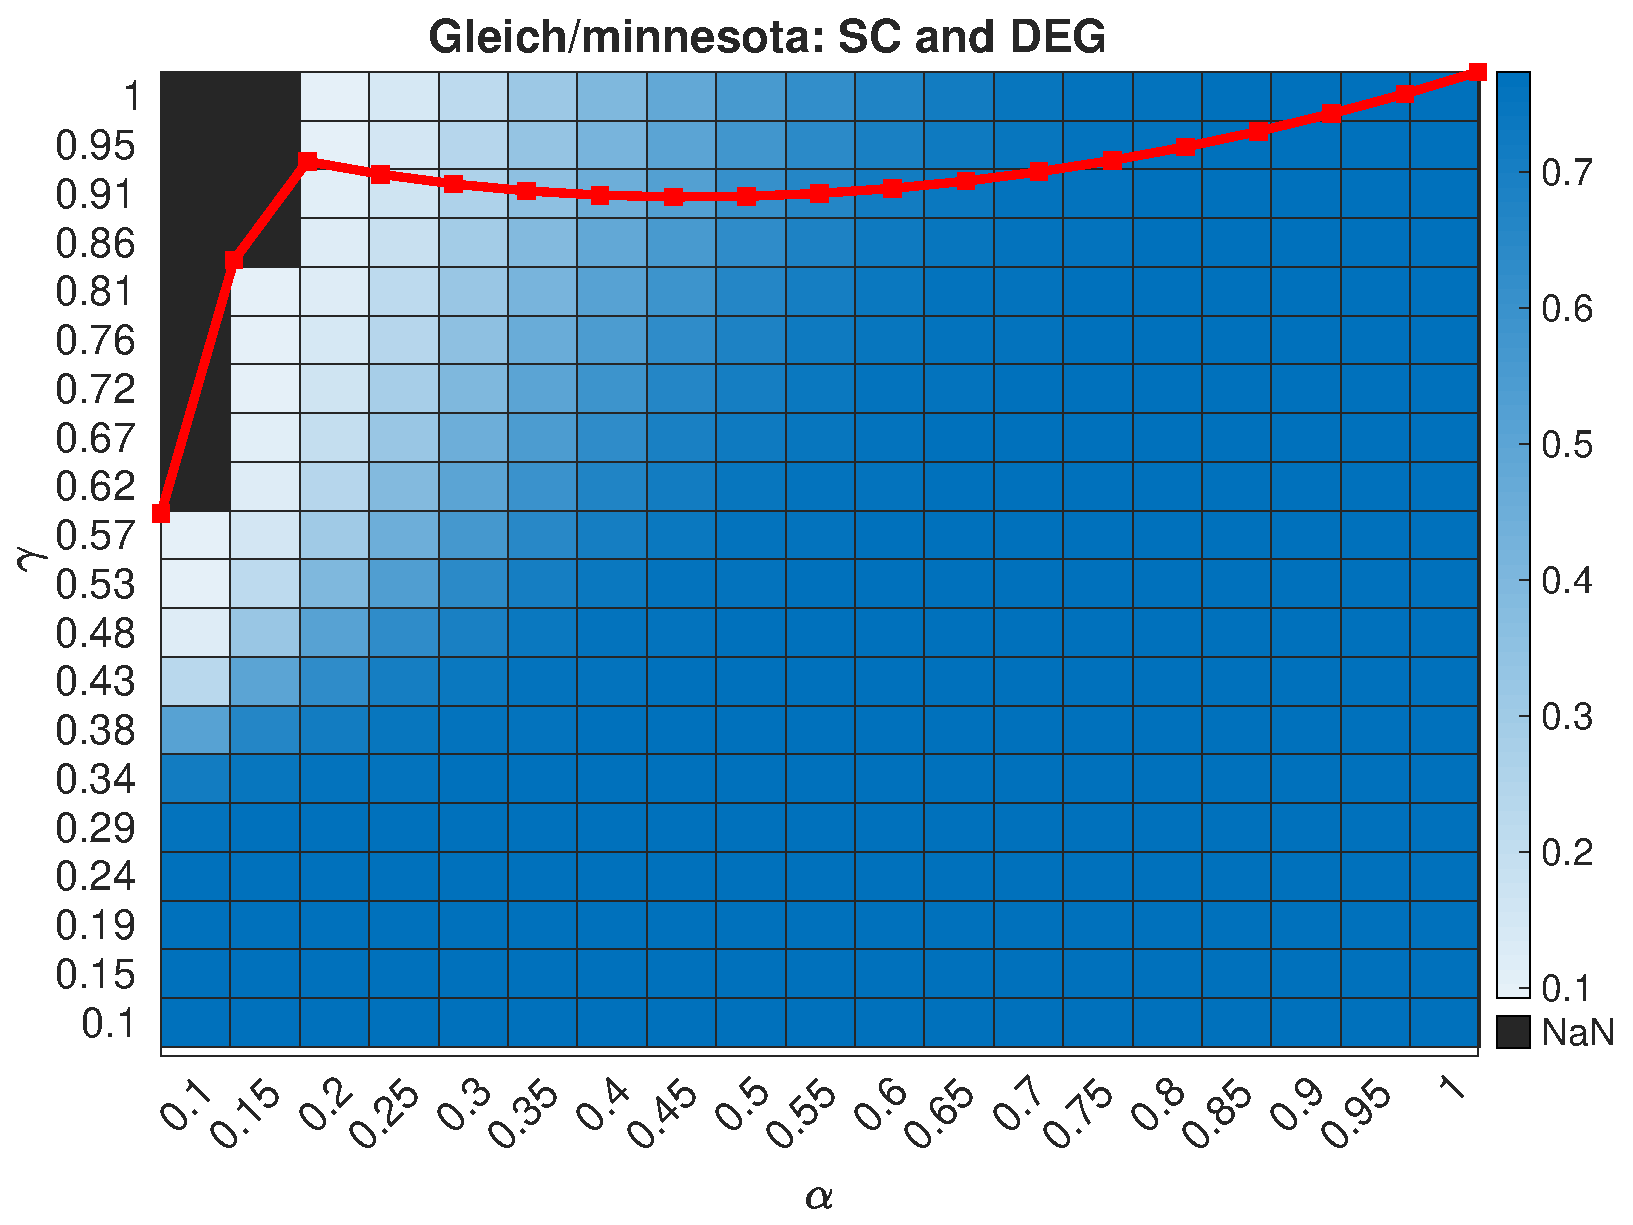
\includegraphics[width=0.7\columnwidth]{Figures/heatmap_SC_deg_minnesota2.eps}}%
\only<2>{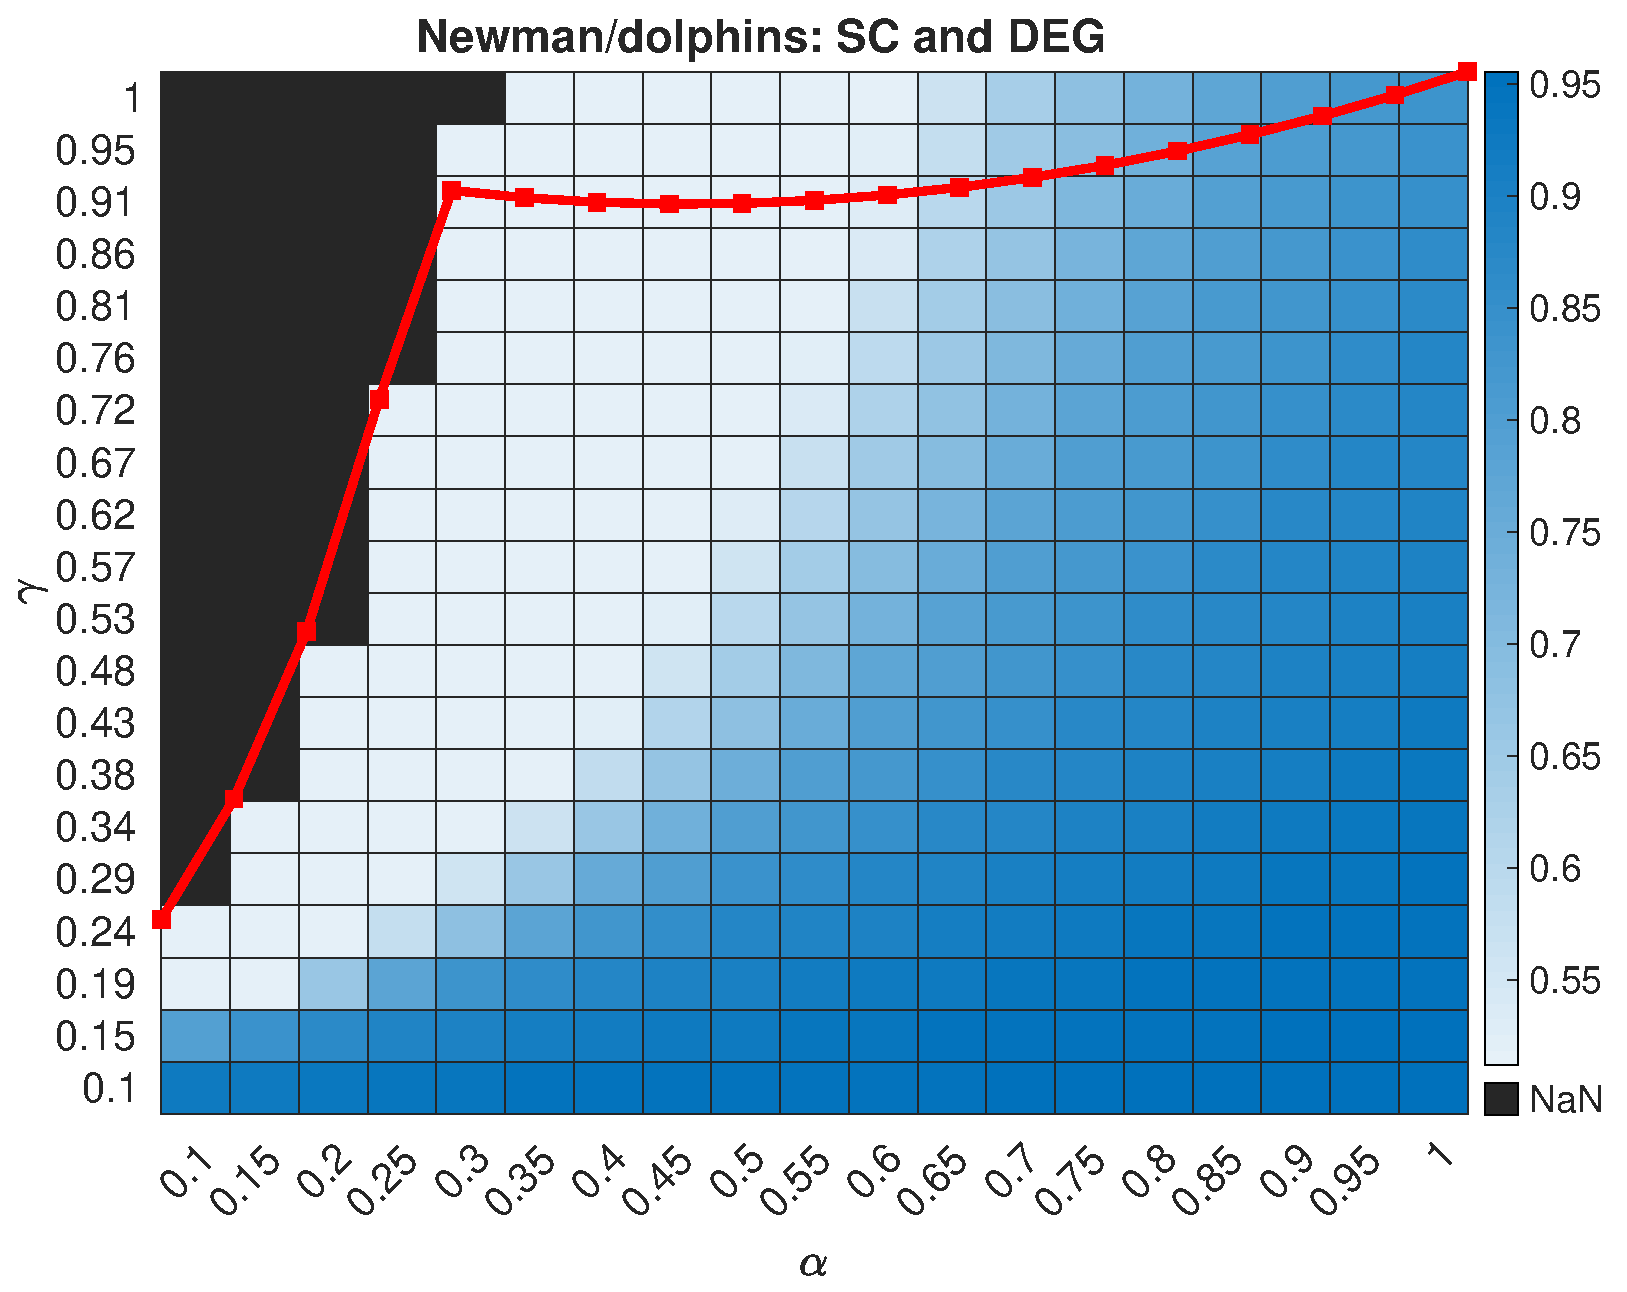
\includegraphics[width=0.7\columnwidth]{Figures/heatmap_SC_deg_dolphins2.eps}}%
\only<3>{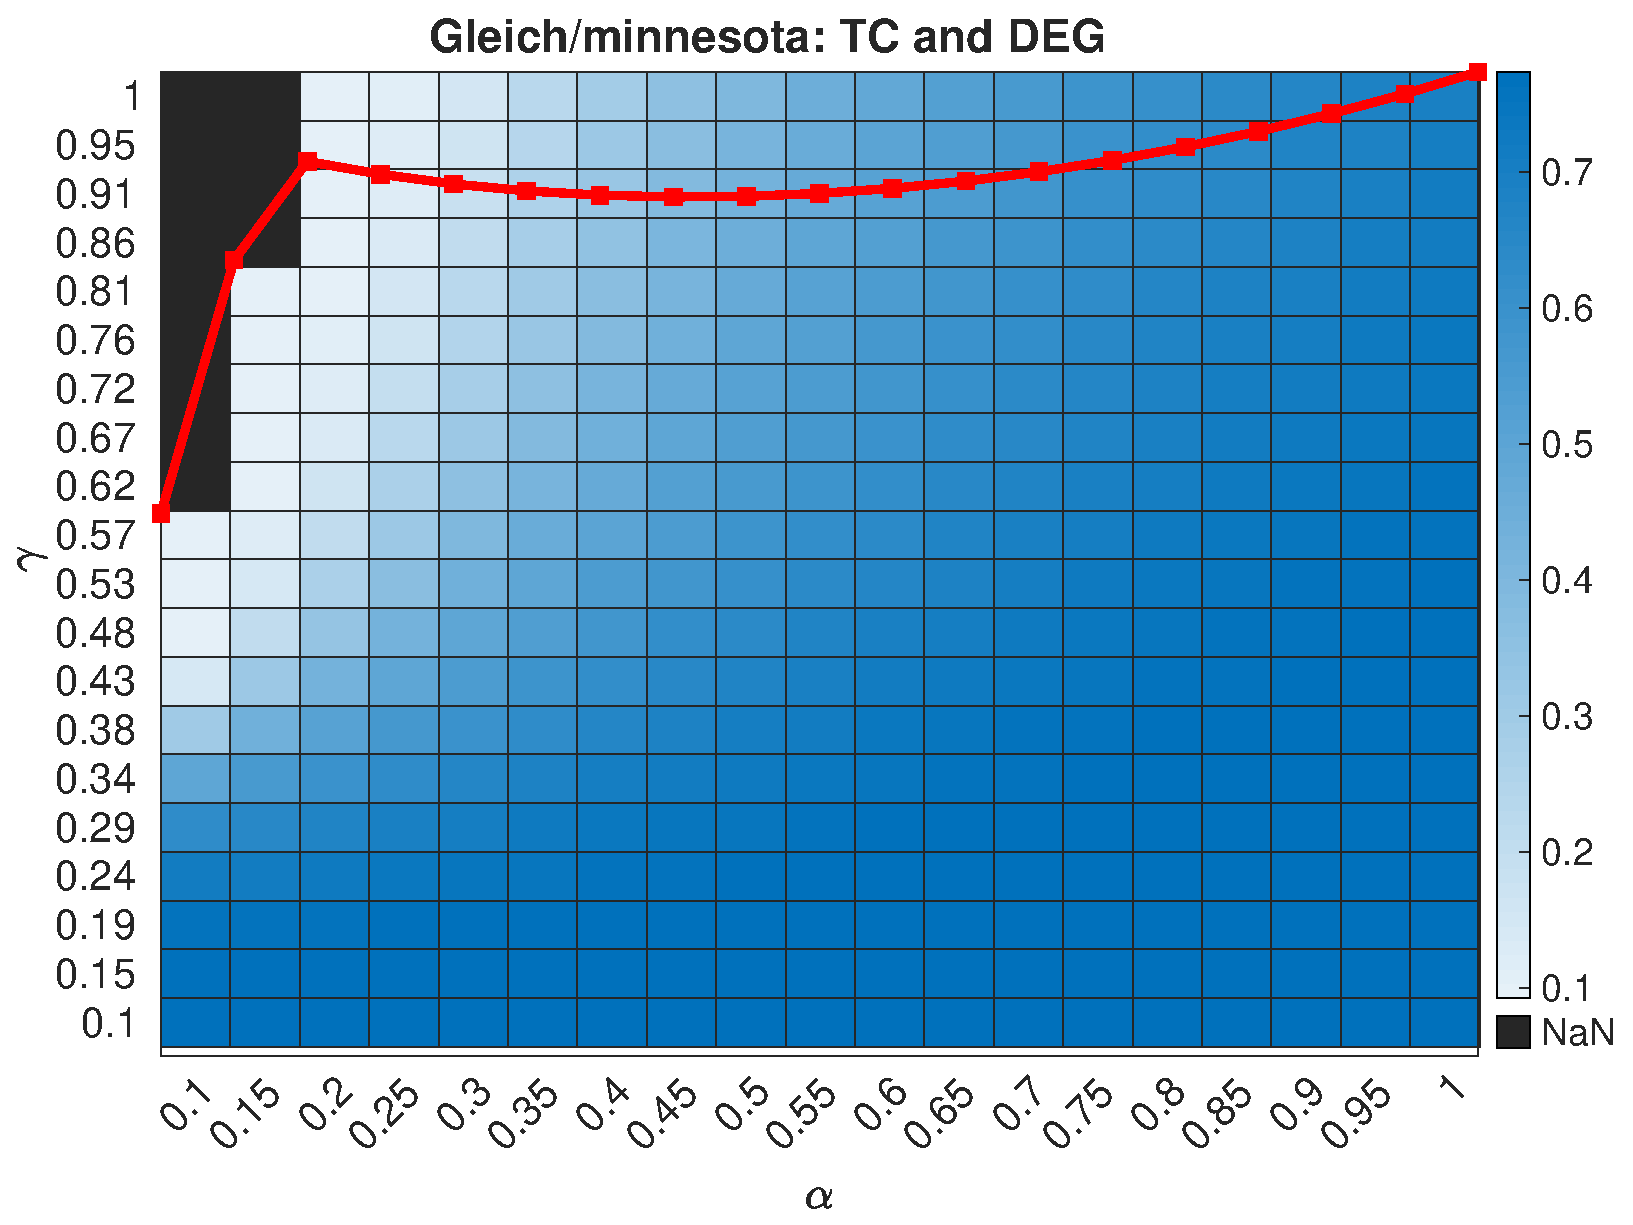
\includegraphics[width=0.7\columnwidth]{Figures/heatmap_TC_deg_minnesota2.eps}}%
\only<4>{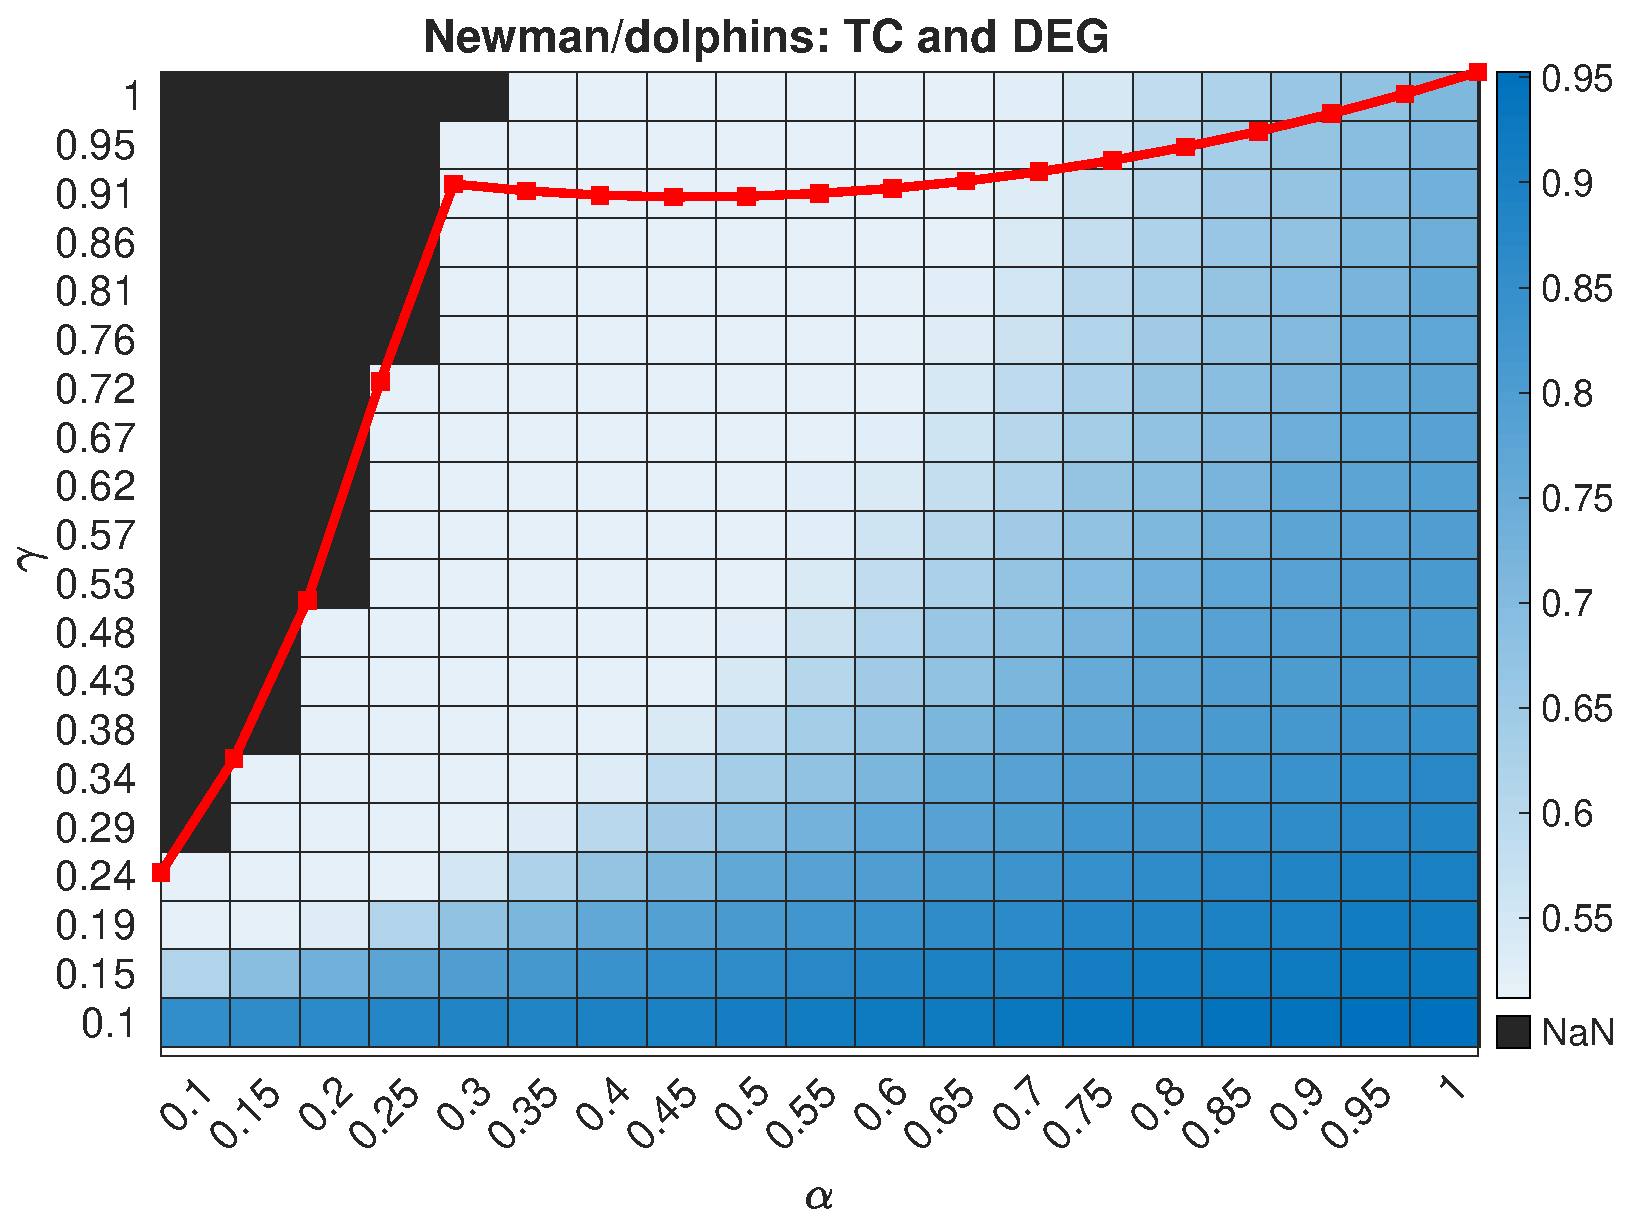
\includegraphics[width=0.7\columnwidth]{Figures/heatmap_TC_deg_dolphins2.eps}}

(a)
\end{column}
\begin{column}{0.5\columnwidth}
\centering\footnotesize

\only<1>{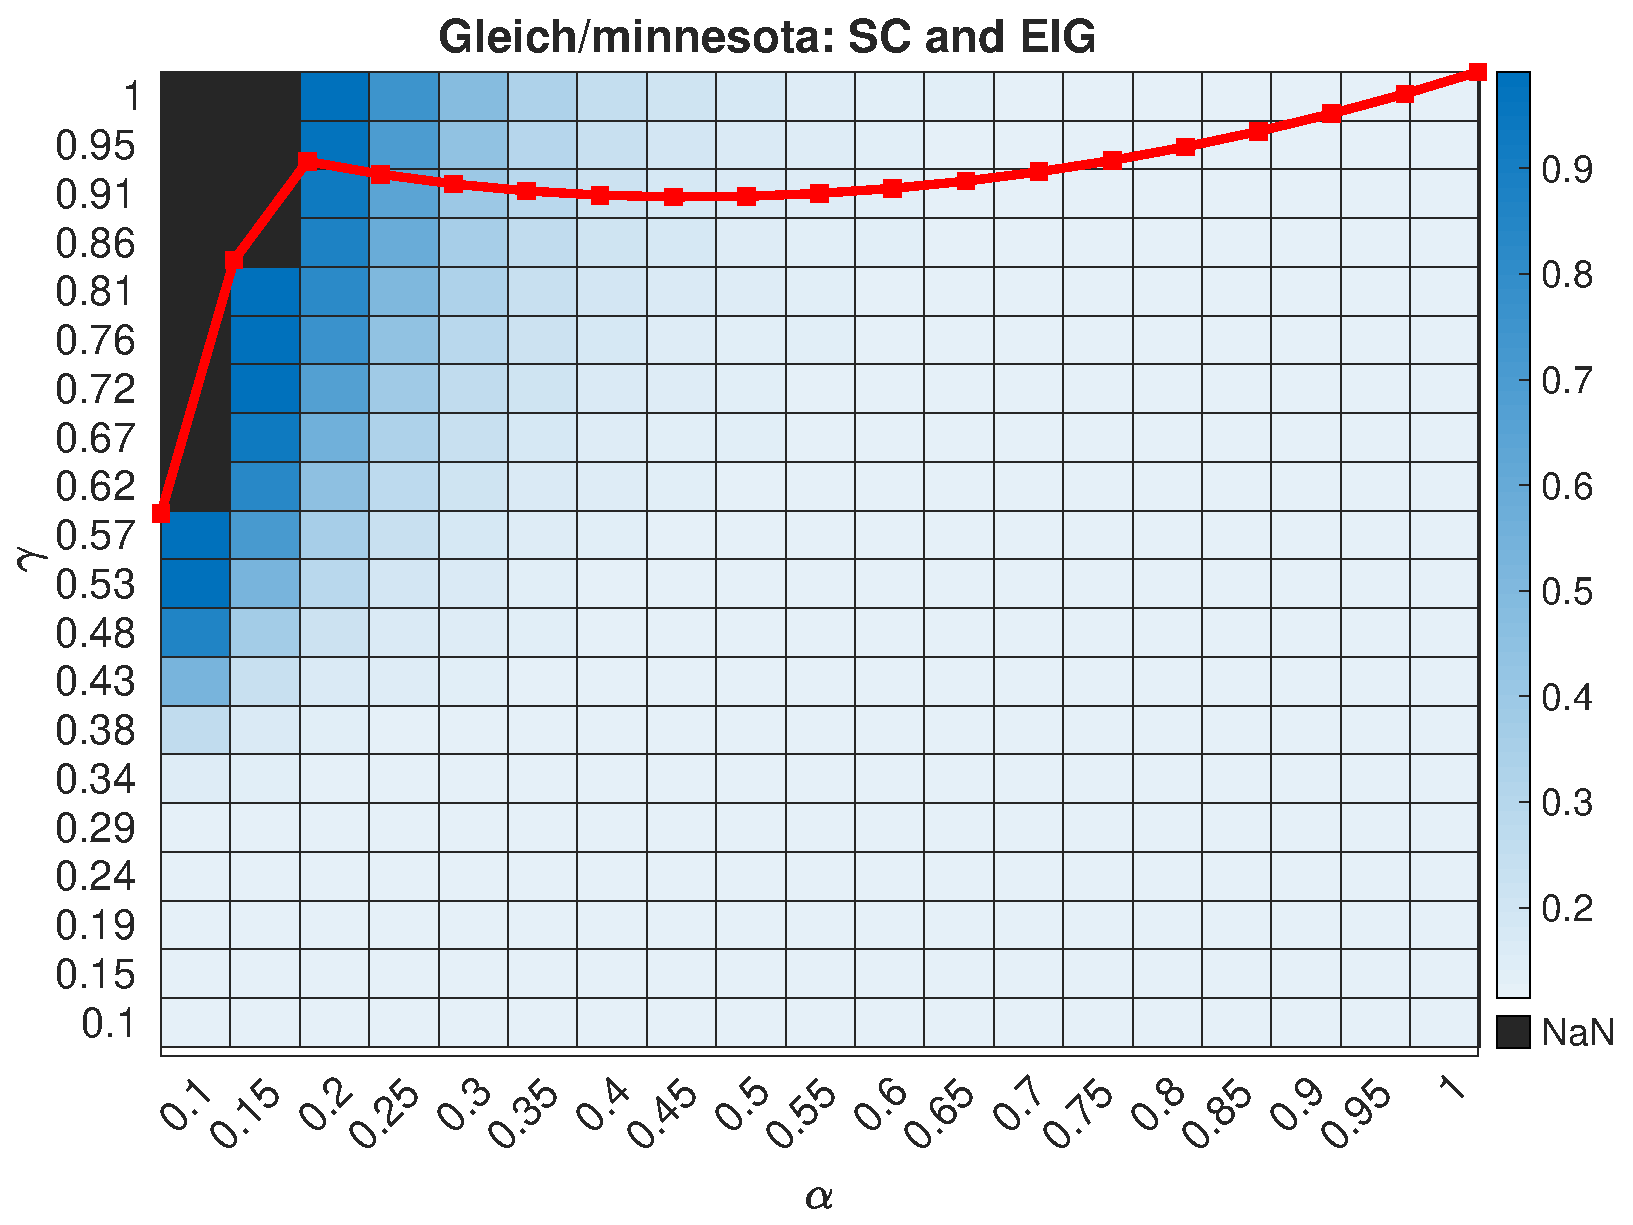
\includegraphics[width=0.7\textwidth]{Figures/heatmap_SC_eig_minnesota2.eps}}%
\only<2>{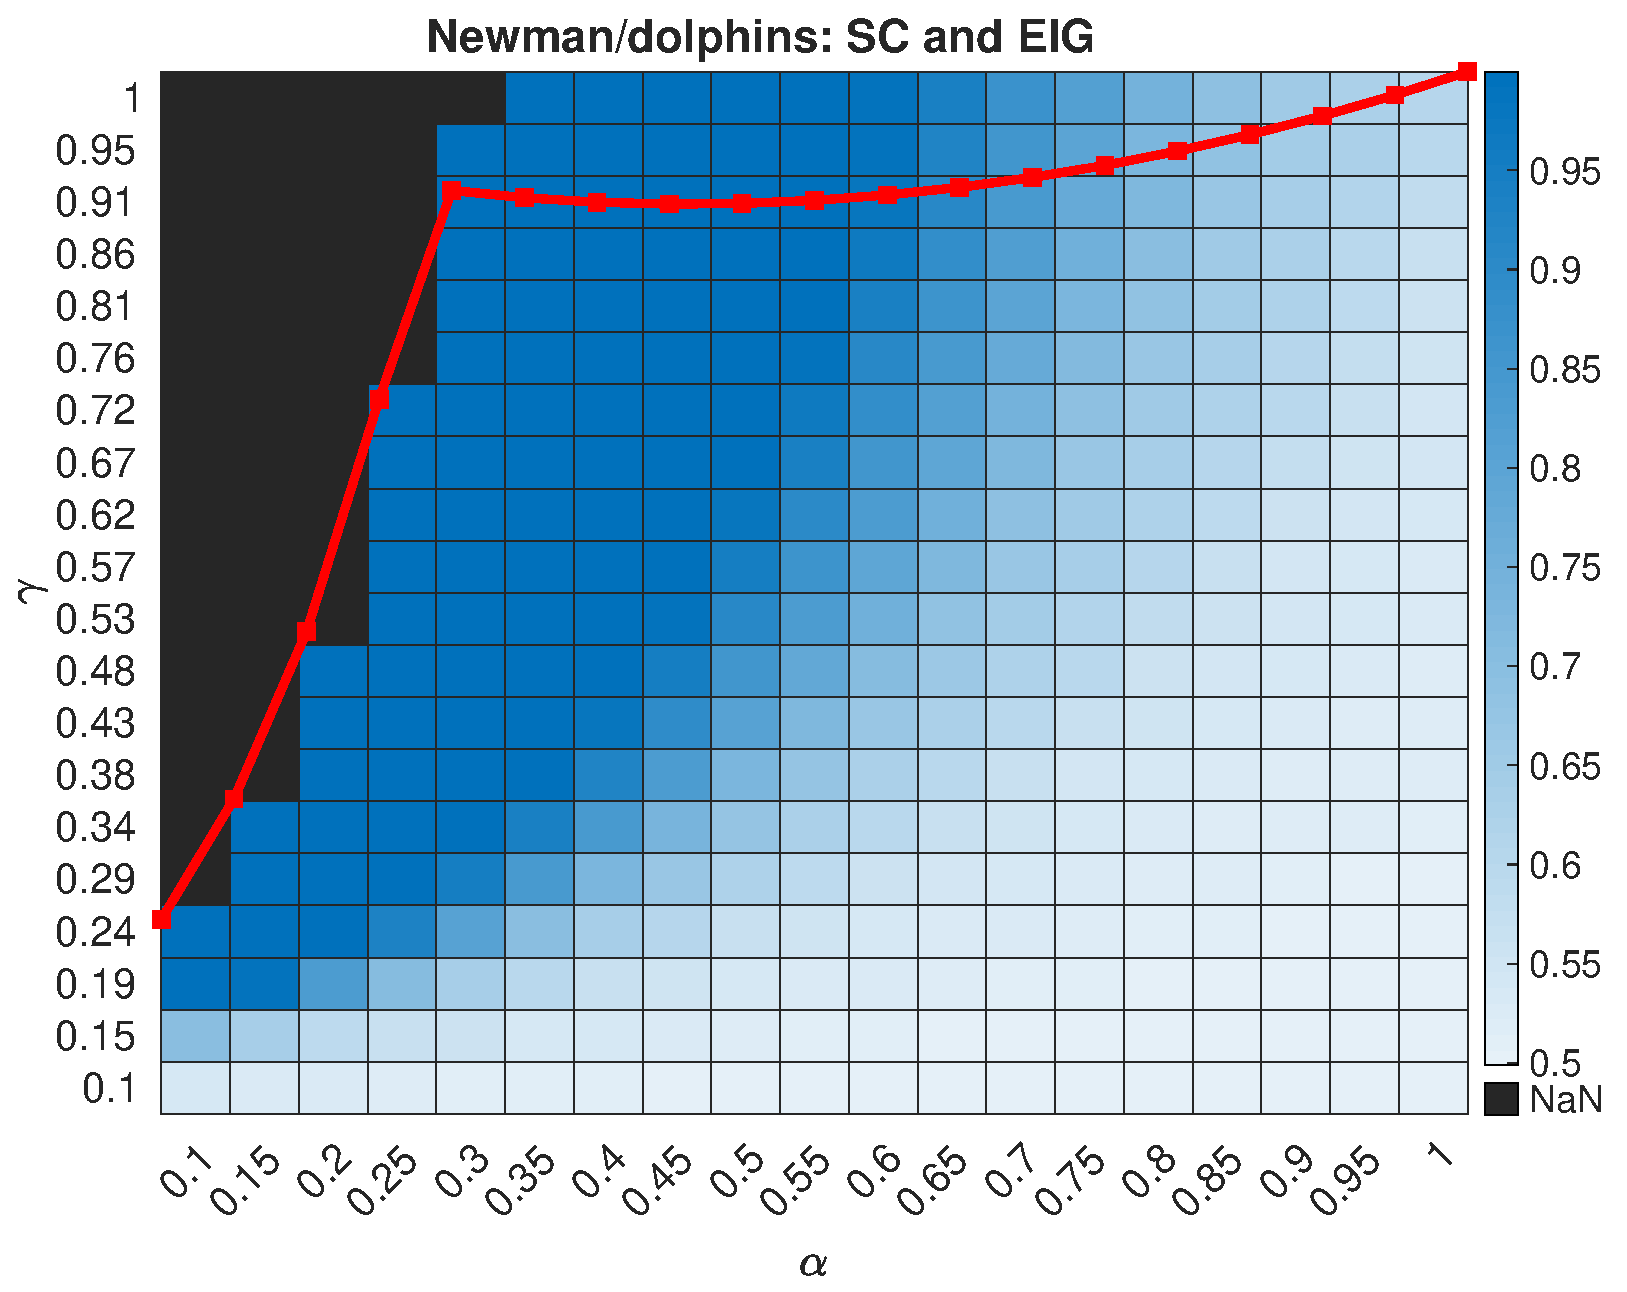
\includegraphics[width=0.7\textwidth]{Figures/heatmap_SC_eig_dolphins2.eps}}%
\only<3>{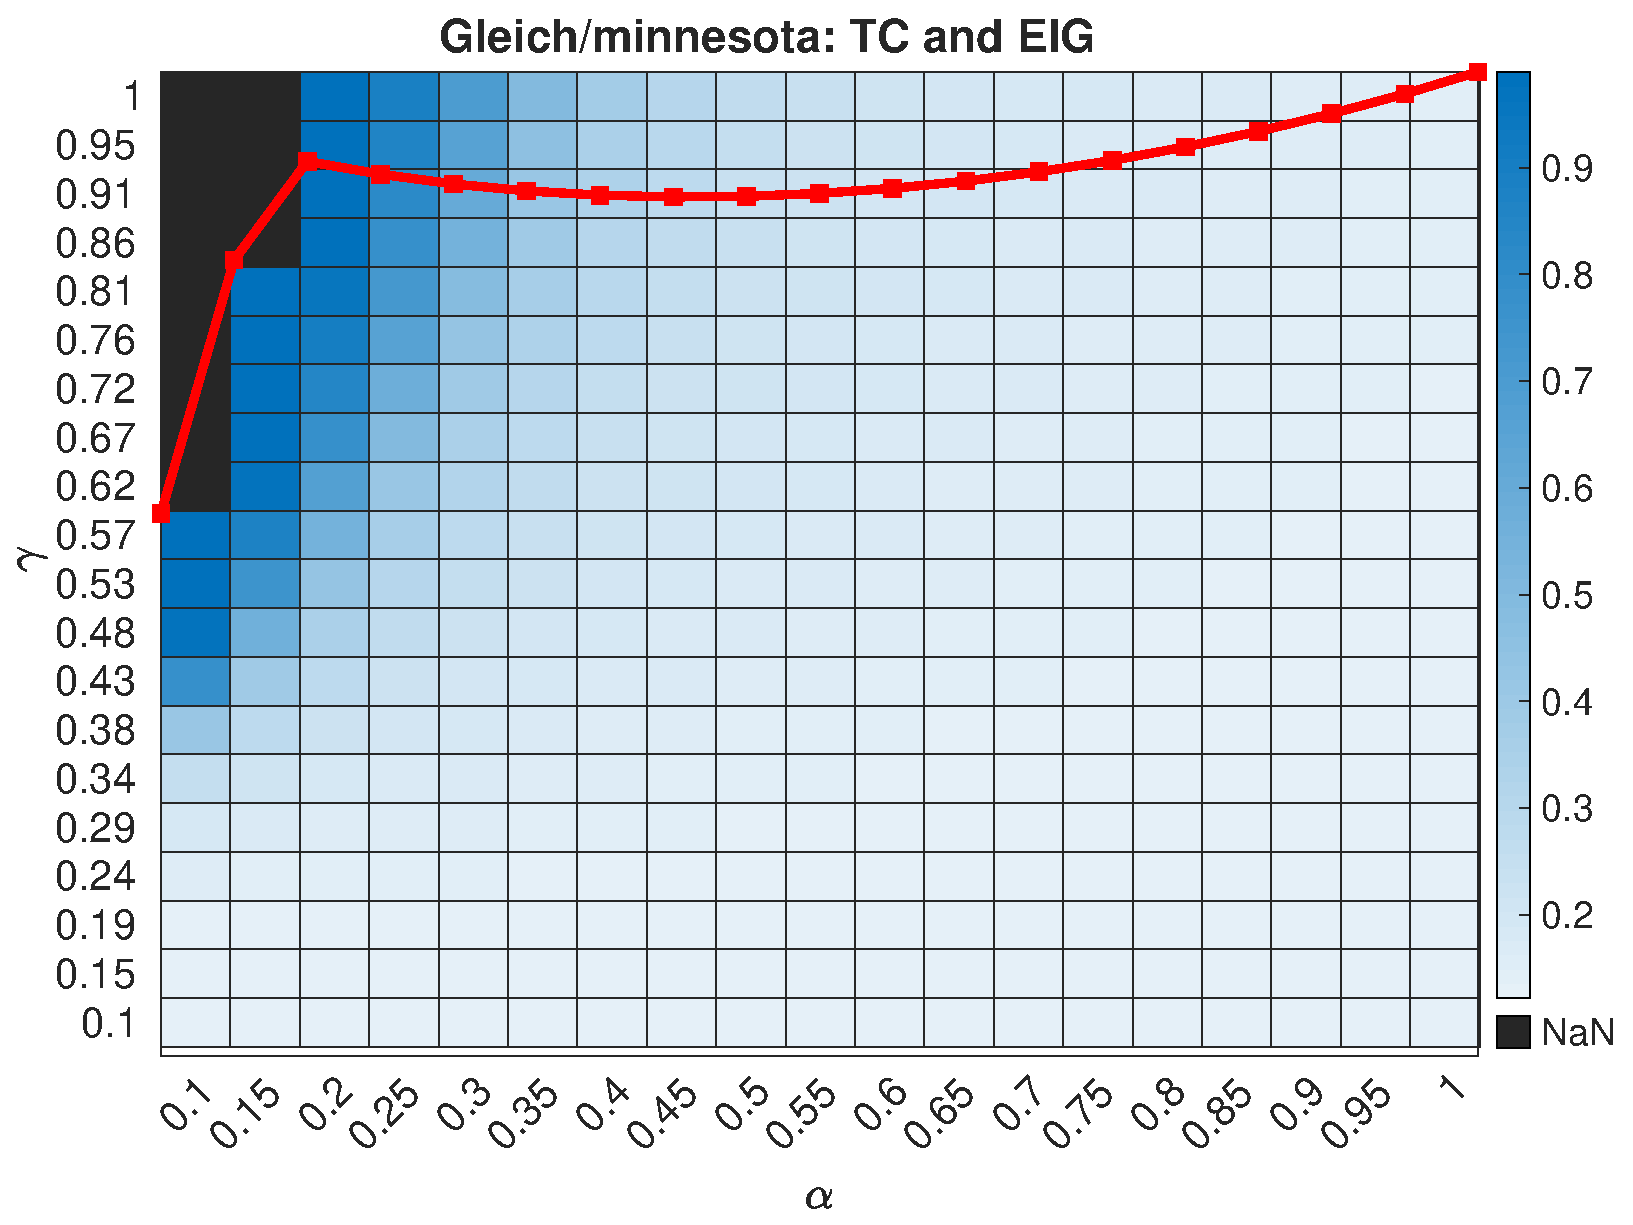
\includegraphics[width=0.7\textwidth]{Figures/heatmap_TC_eig_minnesota2.eps}}%
\only<4>{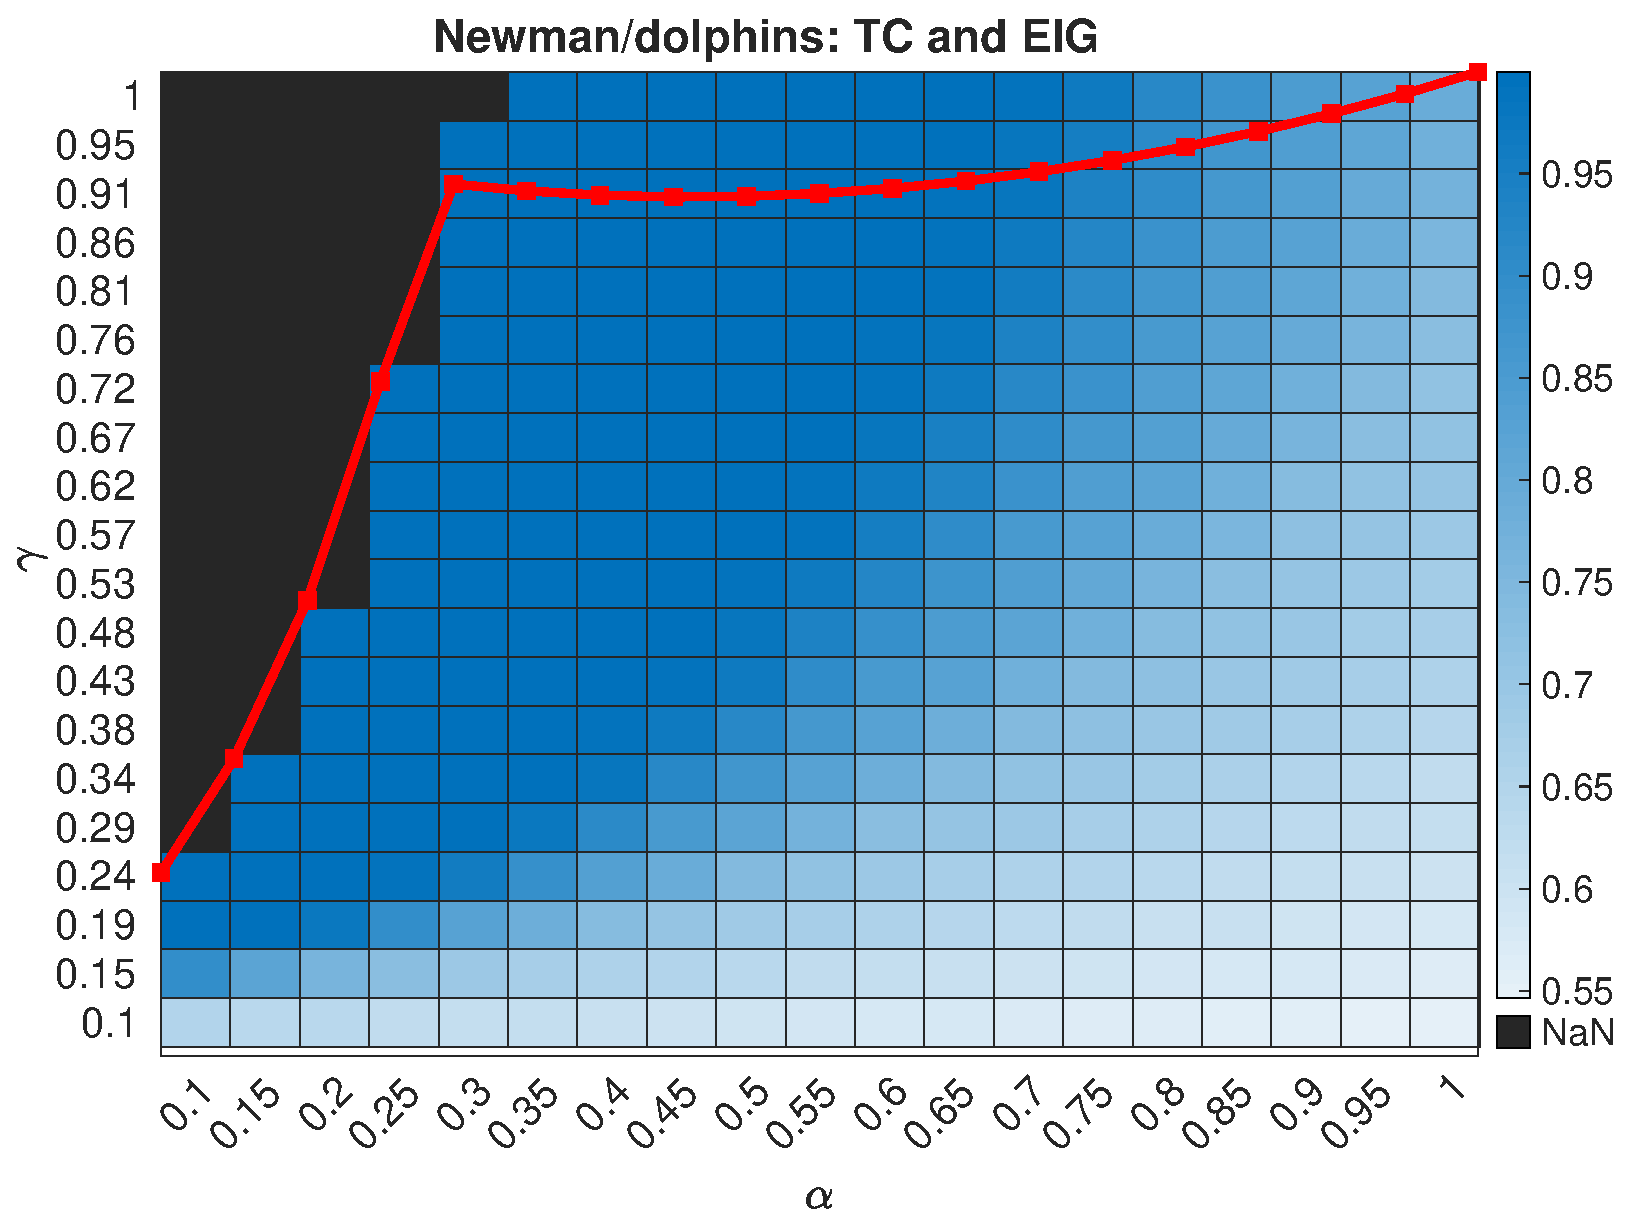
\includegraphics[width=0.7\textwidth]{Figures/heatmap_TC_eig_dolphins2.eps}}

(b)
\end{column}

\end{columns}
\small Kendall correlation coefficient between the ranking induced by total communicability vectors \only<1-2>{$\svec(\widetilde{E}_\alpha)$}\only<3-4>{$\tvec(\widetilde{E}_\alpha)$} and by (a) degree centrality or (b) eigenvector centrality, the red line displays the value of $\mu$.



\end{frame}

\section{Connection with Fractional Calculus}

\begin{frame}{Time-fractional dynamical models on networks}

There are \textbf{several generalizations} of ODE-based models on networks:

\begin{itemize}
	\item[\faFile] Time (and space) generalized diffusion equation on networks~\parencite{DIAZDIAZ2022111791}
	\[
	{}_{CA} D^{\alpha}_{[0,t]}\mathbf{f}(t) = - L \mathbf{f}(t), \quad f(0) = \mathbf{f}_0,
	\]
	for $L$ the \alert{graph Laplacian}, i.e., $L = \operatorname{diag}(A\mathbf{1}) - A$, $A$ adjacency matrix of
	an \emph{undirected graph},
	\item[\faFile] Decision-making models~\parencite{West_2015},
	\item[\faFile] Epidemics modeling with fractional derivative in time on newtorks, e.g.,~\parencite{HUO201641}.
\end{itemize}

\onslide<2>{
There are many more models that involve using \textbf{fractional derivatives with respect to the ``space variables''}, we postpone that discussion after having treated the issue in general for the continuous case.}

\end{frame}

\section{Other types of fractional derivatives w.r.t. time}

\subsection{Distributed order FDEs}

\begin{frame}{Other types of fractional derivatives w.r.t. time}

Another type of FDE w.r.t. that is gaining traction and interest, they are called \textbf{fractional derivatives of distributed order}, i.e.,
\[
\int_{0}^{m} a(r) {}_{CA}D_{[0,t]}^r u(t)\,\mathrm{d}r = f(t), \quad m > 0,
\]
and more generally 
\[
\int_{0}^{m} a(r) F\left( {}_{CA}D_{[0,t]}^r u(t) \right)\,\mathrm{d}r = f(t,u(t)), \quad m > 0.
\]
Applications are, e.g.,
\begin{itemize}
\item[\faFile] Dielectric induction and diffusion \parencite{MR1874477},
\item[\faFile] Kinetic models \parencite{sokolov2004distributed},
\item[\faFile] Distributed-order oscillators \parencite{MR2167221}.
\end{itemize}
\end{frame}

\begin{frame}{Distributed order FDEs}

We can connect them with something we have already seen, consider the \textbf{multi-term} differential equation:
\[
\begin{cases}
\displaystyle \sum_{i=1}^{k} \gamma_i {}_{CA} D^{r_i}_{[0,t]} u(t) = f(t,u(t)), & 0 < r_1 < r_2 < \ldots < r_k \\
u^{(\ell)}(0) = \varphi_\ell, & \ell = 0,\ldots,m-1, \; \displaystyle m = \left\lceil \max_{i=1,\ldots,k} r_i \right\rceil.
\end{cases}
\]
\begin{itemize}
	\item[\faLightbulb] One way of thinking about the distributed-order equation is therefore as the \textbf{limiting case} of with a very 
	large number of terms and where the \alert{coefficients $\gamma_i$ take the values from the function $a$}. 
	\item[\faQuestionCircle]<2-> What can we say about the solutions?
\end{itemize}

\end{frame}

\begin{frame}{Distributed order FDEs}

For the \textbf{linear case} 
\begin{equation}\label{eq:linearFDE}
\int_{0}^{m} a(r) {}_{CA}D_{[0,t]}^r u(t)\,\mathrm{d}r = f(t), \quad m > 0, \tag{LDFODE}
\end{equation}
we can prove existence under some \emph{assumptions}:
\begin{itemize}
\item[(A1)] $m \in \mathbb{N}$,
\item[(A2)] $a$ is \emph{absolutely integrable} on $[0,m]$ with $\int_{0}^{m} a(r) s^r\,\mathrm{d}r \neq 0$ for $\Re(s) > 0$,
\item[(A3)] $f \in \mathbb{L}^1([0,\infty)]$,
\item[(A4)] $u$ is such that ${}_{CA} D^{r}_{[0,\infty)} u(t)$ for $t \in [0,+\infty)$ for $r \in [0,m]$.
\end{itemize}
\only<2-5>{
We apply Laplace transform\only<3->{, then use (A4) and exchange the transform and the integral}\only<5->{. After rearranging and inverting using (A1)--(A3)}
\only<2>{\[
\mathcal{L}\left\lbrace \int_{0}^{m} a(r) {}_{CA}D_{[0,t]}^r u(t)\,\mathrm{d}r \right\rbrace(s) = \mathcal{L}\left\lbrace f \right\rbrace(s)
\]}
\only<3>{\[
\int_{0}^{m} a(r) \mathcal{L}\left\lbrace {}_{CA}D_{[0,t]}^r u \right\rbrace(s)\,\mathrm{d}r = \mathcal{L}\left\lbrace f \right\rbrace(s)
\]}
\only<4>{
\[
\int_{0}^{m} a(r) \left( s^r \mathcal{L}\{u\}(s) - u(0)s^{r-1} \right) \,\mathrm{d}r - \sum_{j=1}^{m-1} \int_{j}^{m} a(r) u^{(j)}(0) s^{r-j-1}\,\mathrm{d}r = \mathcal{L}\left\lbrace f \right\rbrace(s)
\]
}
\only<5>{\[
u(t) = u(0) + \left(f * \mathcal{L}^{-1}\left\lbrace \frac{1}{\int_{0}^{m} a(z)(s)^z\,\mathrm{d}z } \right\rbrace \right)(t) + \sum_{j=1}^{m-1} u^{(j)}(0) \mathcal{L}^{-1} \left\lbrace \frac{\int_{j}^{m} a(r) s^{r-j-1}\,\mathrm{d}r }{ \int_{0}^{m} s^r a(r)\,\mathrm{d}r } \right\rbrace(t).
\]}
}
\begin{onlyenv}<6>
\begin{alertblock}{Theorem~\parencite[Theorem~3.1]{DIETHELM200996}}
Under assumptions (A1)--(A4) on $a$, $f$ and $u$, \eqref{eq:linearFDE} has a unique solution. 
\end{alertblock}
\end{onlyenv}

\end{frame}

\begin{frame}{Properties of the \eqref{eq:linearFDE} solution}

\begin{alertblock}{Proposition~\parencite{DIETHELM200996}}
\begin{enumerate}
\item Under assumptions (A1)--(A4) and for fixed $T > 0$ the solution to \eqref{eq:linearFDE} satisfies $u^{(m)}(t)$ is bounded and measurable in $[0,T]$.
\item Let $u \in \mathcal{C}^p([O,T])$ with some $p \in \mathbb{N}$ and $T > 0$. For every fixed $t \in [0,T]$, consider ${}_{CA}D_{[0,t]}^r u(t) = z(r)$ as a function of $r$. Then,
\begin{itemize}
	\item \normalsize At the integer argument $j=1,2,\ldots,p-1$ the function $z$ has a \emph{jump discontinuity} that can be described as
	\[
	\lim_{r \rightarrow j^+} z(r) - \lim_{r \rightarrow j^-} z(r) = - u^{(j)}(0).
	\]
	\item \normalsize There exist a \emph{continuous transition} iff $u^{(j)}(0) = 0$.
\end{itemize}
\end{enumerate}
\end{alertblock}

\onslide<2>{
\begin{center}
\faQuestionCircle\, How can we discretize and solve this type of equations?
\end{center}
}

\end{frame}

\begin{frame}{Discretization strategies}

\begin{enumerate}
\item<1-> We discretize the \textbf{integral term} in the \textbf{distributed-order} equation
\begin{itemize} 
	\item[\faCog]<2-> Fix $\phi(z) = a(z) {}_{CA}D_{[0,t]}^z u(t)$ and use a quadrature formula
	\[ \int_{0}^{m} \phi(z)\,\mathrm{d}z \approx \sum_{j=0}^{n} w_j \phi(z_j) \]
	\alert{\faExclamationTriangle} Every integer value in the interval $[0,m]$ is a $z_j$, in
	general every $z_j \in \mathbb{Q}$.
\end{itemize}
\item<1-> We solve the multi-term equation
	\begin{itemize}
	\item[\faCog]<3-> With the choice we have made we now have a multiterm equation of the form
	\[
	\sum_{j=0}^{n} w_j a(z_j) {}_{CA}D^{z_j}_{[0,t]} u(t) = f(t), \quad z_1 < z_2 < \ldots < z_n,
	\]
	\item[\faCog]<4-> We apply the reformulation as a system of equations of order $q$ being
	the \textbf{g}reatest \textbf{c}ommon \textbf{d}ivisor of the derivative orders.
	\end{itemize}
\end{enumerate}

\end{frame}

\begin{frame}{Error analysis}
To select the \textbf{quadrature formula} we have to take into account the \textbf{jumps in the integrand}
\[
\int_{0}^{m} a(r) {}_{CA}D^r_{[0,t]}u(t)\,\mathrm{d}r = \sum_{i=0}^{m-1} \int_{i}^{i+1} a(r) {}_{CA}D^r_{[0,t]}u(t)\,\mathrm{d}r = \sum_{i=0}^{m-1} \sum_{j=0}^{n_i} w_{ij} a(z_{ij}) {}_{CA}D^{z_{ij}}_{[0,t]}u(t)
\]
with
\begin{itemize}
	\item[\faCog]<1-> $z_{i0} = i$, $z_{i,n_i} = i+1$, $\forall i$,
	\item[\faCog]<2-> $j=0$, $j=n_{i}$ the expressions ${}_{CA}D^{z_{ij}}_{[0,t]}u(t)$ must be interpreted as
	\begin{align*}
	\lim_{s \rightarrow z_{i0}^+} {}_{CA}D^{s}_{[0,t]}u(t) = & \lim_{s \rightarrow i^+} {}_{CA}D^{s}_{[0,t]}u(t), \\
	\lim_{s \rightarrow z_{in_i}^-} {}_{CA}D^{s}_{[0,t]}u(t) = & \lim_{s \rightarrow (i+1)^-} {}_{CA}D^{s}_{[0,t]}u(t).
	\end{align*}
	\item[\faCog]<3-> The sequence $\{z_j\} = \{ z_0 = z_{00}, z_{1} = z_{01}, \ldots, z_{n_0} = z_{0n_0} = z_{10} = 1, \ldots \}$.
\end{itemize}

\end{frame}

\begin{frame}{Error analysis}

To proceed further we also need to require further regularity on the $a$ function. 

We assume
\begin{itemize}
\item[(Q1)] We use a convergent quadrature rule of order $p > 0$,
\item[(Q2)] For all $i$, the weights of the quadrature rule are bounded by
\[
C_1 n_i^{-1} \leq \min_{j=0,1,\ldots,n_i} |w_{ij}| \leq \max_{j=0,1,\ldots,n_i} |w_{ij}| \leq C_2 n_i^{-1},
\]
with some constants $C_1$ and $C_2$.
\item[(Q3)] The function $a$ is \alert{$p$-times continuously differentiable} on $[0,m]$.
\end{itemize}

\begin{alertblock}{Proposition \parencite{DIETHELM200996}}
If $\tilde{u}$ is the solution of \eqref{eq:linearFDE} obtained using a quadrature formula satistying (Q1)--(Q4), then
\[
u(t) = \tilde{u}(t) + O( \max_{i} \{ n_i^{-p} \} ), \qquad \text{ for } n_i \rightarrow +\infty \; \forall\,i. 
\]
\end{alertblock}

\end{frame}

\begin{frame}{Error analysis}

Thus, if we assume that we apply a numerical method for the multi-term equation which has order of convergence $O(\tau^q)$ we have then
\begin{alertblock}{Theorem \parencite[Theorem~4.1]{DIETHELM200996}}
Under the conditions (A1)--(A4), (Q1)--(Q3), the overall error of the proposed algorithm for~\eqref{eq:linearFDE} satisfies for $j\tau \in [0,T]$:
\[
\max\{ |u_j - u(j\tau) |\;:\; j \geq 0, \; j\tau \leq T \} = O(\tau^q) + O( \max_{i} \{ n_i^{-p} \} ) \qquad \text{ for } n_i \rightarrow +\infty \; \forall\,i, \; \tau \rightarrow 0.
\]
\end{alertblock}

\begin{itemize}
\item[\faWrench] To reduce the number of terms and the regularity requirements on $a$ one could use a Gauss-type quadrature built explicitely for the given function $a(z)$ (that now needs to be only continuous) \parencite{MR4015149}.
\end{itemize}

\end{frame}

\subsection{Variable order FDEs}

\begin{frame}{Variable order FDEs}

Consider a function $\alpha\,:\,[0,T] \subset \mathbb{R}^+ \rightarrow (0,1)$ we can think of generalizing the Riemann-Liouville integral as
\[
I_{[0,t]}^{\alpha(t)} = \frac{1}{\Gamma(\alpha(t))} \int_{0}^{t} (t-\tau)^{\alpha(t)-1} f(\tau)\,\mathrm{d}\tau,
\]
possibly coupled with the Riemann-Liouville variable-order derivative
\[
{}_{RL}D_{[0,t]}^{\alpha(t)} = \frac{1}{\Gamma(1-\alpha(t))} \frac{d}{dt} \int_{0}^{t} (t-\tau)^{-\alpha(t)} f(\tau)\,\mathrm{d}\tau,
\]
\onslide<2->{

\alert{\faExclamationTriangle}  The \textbf{characterization} of fractional calculus
\textbf{based} on \textbf{these operators} is rather \alert{\textbf{problematic}} since ${}_{RL}D_{[0,t]}^{\alpha(t)}$ is \alert{\textbf{not a left-inverse}} of $I_{[0,t]}^{\alpha(t)}$; see~\parencite{MR1349652}.

}

\onslide<3>{

Some of this generalizations have found use in physical modeling, but they are \emph{problematic from a rigorous point of view}.

}
\end{frame}

\begin{frame}{Variable order FDEs a Laplace domain version}

Among the first ideas in developing a time-variable time-fractional calculus there are three seminal works by \textbf{Giambattista Scarpi}
\begin{itemize}
\item[\faFile] G. Scarpi, Sopra il moto laminare di liquidi a viscosist variabile nel tempo. Atti Accademia delle Scienze, Isitituto di Bologna, Rendiconti (Ser XII), 9 (1972), pp. 54-68,
\item[\faFile] G. Scarpi, Sulla possibilità di un modello reologico intermedio di tipo evolutivo. Atti Accad Naz Lincei Rend Cl Sci Fis Mat Nat (8), 52 (1972), pp. 912-917;
\item[\faFile] G. Scarpi, Sui modelli reologici intermedi per liquidi viscoelastici. Atti Accad Sci Torino: Cl Sci Fis Mat Natur, 107 (1973), pp. 239-243.
\end{itemize}

Recently, this approach has been taken again into account to overcome the limitation given by the \emph{naive} replacement of the $\alpha(t)$ function in the kernel of Fractional Integrals and Derivatives; \parencite{MR4268683}.

\end{frame}

\begin{frame}{Scarpi's Derivative~{\Large\parencite{MR4268683}}}
To introduce this new version we need to use again the \textbf{Laplace transform} of the Caputo derivative and Riemann-Liouville integrals
\[
\mathcal{L}\{ {}_{CA}D^{\alpha}_{[0,t]} f(t) \}(s) = s^\alpha F(s) - s^{\alpha-1} f(0), \quad \mathcal{L}\{ I^{\alpha}_{[0,t]} f(t) \}(s) = \frac{1}{s^\alpha}F(s),
\]
and consider a \textbf{locally integrable} function $\alpha(t)\,:\,[0,T] \rightarrow (0,1)$ .

\begin{exampleblock}<2->{\faLightbulb\;Scarpi's idea}
If $\alpha(t) \equiv \alpha$, $t > 0$, $\mathcal{L}{\alpha}(s) = A(s) = \nicefrac{\alpha}{s}$, then
\[
\mathcal{L}\left\lbrace \frac{t^{-\alpha}}{\Gamma(1-\alpha)} \right\rbrace(s) = s^{s A(s) - 1} = s^{\alpha-1} \qquad \mathcal{L}\left\lbrace \frac{t^{\alpha-1}}{\Gamma(\alpha)} \right\rbrace(s) = s^{- s A(s)} = \frac{1}{s^\alpha}.
\]
\faLightbulb\;Apply the same relation to any $\alpha(t)$ with $A(s) = \mathcal{L}\{\alpha(t),s\} = \int_{0}^{+\infty} e^{-st} \alpha(t)\,\mathrm{d}t$.
\end{exampleblock}

\end{frame}

\begin{frame}{Scarpi's Derivative~{\Large\parencite{MR4268683}}}\vspace{-0.5em}

\begin{block}{Scarpi Fractional Derivative}
Let $\alpha(t)\,:\,[0,T] \rightarrow (0,1)$ be a locally integrable function with Laplace transform $A(s)$, and let $f \in \mathbb{L}^{1}([0,T])$. We define the Scarpi fractional derivative ${}_{S}D^{\alpha(t)}_{[0,t]}$ of variable order $\alpha(t)$ as\vspace{-0.5em}
\[
{}_{S}D^{\alpha(t)}_{[0,t]} f(t) = \frac{d}{d t} \int_{0}^{t} \phi_\alpha(t-\tau) f(\tau)\,\mathrm{d}\tau - \phi_\alpha(t)f(0), \qquad t \in (0,T],
\]
where the kernel function $\phi_a(t)$ is the inverse Laplace transform
\[
\phi_a(t) = \mathcal{L}^{-1} \left\lbrace \Phi_\alpha(s) \right\rbrace (t), \qquad \Phi_\alpha(s) = s^{s A(s) - 1}.
\]
\end{block}

\begin{alertblock}<2->{Proposition \parencite[Proposition~2.1]{MR4268683}}
Let $\alpha(t)\,:\,[0,T] \rightarrow (0,1)$ be a locally integrable function with Laplace transform $A(s)$, let $\phi_\alpha(t)$ be the inverse Laplace transform of $\Phi_\alpha(s) = s^{s A(s)-1}$, if $f \in \mathbb{A}([0,T])$ then\vspace{-1em}
\[
{}_{S}D^{\alpha(t)}_{[0,t]} f(t) = \int_{0}^{t} \phi_\alpha(t-\tau) f'(\tau)\,\mathrm{d}\tau, \qquad t \in [0,T].
\]
\end{alertblock}

\end{frame}

\begin{frame}{Scarpi's Integral~{\Large\parencite{MR4268683}}}
To ``fix'' the behavior of the naive definition we need also the related formulation of the fractional integral, that is having an operator for which
\[
{}_{S}D^{\alpha(t)}_{[0,t]} {}_{S}I^{\alpha(t)}_{[0,t]}f(t) = f(t) \qquad  I^{\alpha(t)}_{[0,t]}{}_{S}D^{\alpha(t)}_{[0,t]} f(t) = f(t)-f(0),
\]
Going there-and-back the Laplace domain can be rewritten as the \textbf{Sonine condition}\vspace{-0.5em}
\[
\int_{0}^{t} \phi_\alpha(t-\tau) \psi_\alpha(\tau) = 1, \qquad t > 0.
\]\vspace{-0.5em}
\begin{block}<2->{Scarpi Fractional Integral} 
Let $\alpha\,:[0,T]\rightarrow (0,1)$ be a locally integrable function with Laplace transform $A(s)$, let $f \in \mathbb{L}^1([0,T])$ we define the Scarpi fractional integral as\vspace{-0.5em}
\[
{}_{S}I^{\alpha(t)}_{[0,t]}f(t) = \int_{0}^{t} \psi_\alpha(t-\tau)f(\tau)\,\mathrm{d}\tau,
\]
with $\psi_\alpha(t) = \mathcal{L}^{-1}\left\lbrace \Psi_\alpha(s)\right\rbrace(t)$ for $\Psi_\alpha(s) = s^{-s A(s)}$.
\end{block}

\end{frame}

\begin{frame}{Finding good $\alpha(t)$~{\Large\parencite{MR4268683}}}

In principle not all transition functions $\alpha(t)$ will allow for a suitable definition of a pair of Scarpi's operators.

\begin{description}
\item[Necessary condition]<2-> A necessary requirement to ensure that $\phi(t)$ and $\psi(t)$ form a \textbf{Sonine pair} is for them to have an
integrable singularity at the origin. 
two functions 
\item[Reality]<3-> we also want our Kernels to be real, but this follows from having a real $\alpha(t)$ and hence $\overline{A(\overline{s})} = A(s)$,
\item[Kernels are LT]<4-> a necessary conditions to have $\Phi_\alpha(s)$ and $\Psi_\alpha(s)$ Laplace transform of two functions $\phi_\alpha(t)$ and $\psi_\alpha(t)$ is to require
\[
\lim_{t \rightarrow 0^+} \alpha(t) = \overline{\alpha} \in (0,1)
\]
and then the \textbf{initial value Theorem for the Laplace transform} ensures that $\{\Phi_\alpha,\Psi_\alpha\} \rightarrow 0$ for $s \rightarrow +\infty$, and thus they are the LT transform of two functions.
\item[$\Rightarrow$]<5-> Any function $\alpha(t)$ with LT $A(s)$ is suitable provided tha $\Phi_\alpha(s)$ and $\Psi_\alpha(s)$ are LTs of some functions.
\end{description}

\end{frame}

\begin{frame}{Solving FDEs with Scarpi's Derivative}

Consider the case
\[
\begin{cases}
{}_{S}D^{\alpha(t)}_{[0,t]} y(t) = -\lambda y(t), \\
y(0) = y_0
\end{cases} \qquad \mathbb{R} \ni \lambda > 0
\]
\begin{enumerate}
\item<2-> We apply Laplace transform on both sides
\[
s^{sA(s)} Y(s) - s^{s A(s) - 1} y_0 = -\lambda Y(s)
\]
where $Y(s) = \mathcal{L}\{y(t)\}(s)$
\item<3-> Solve for $Y(s)$
\[
Y(s) = \frac{y_0}{s(1 + \lambda \Psi_\alpha(s))},
\]
\item<4-> \textbf{Numerically invert the Laplace transform} with one of the algorithms we have seen when discussing the computation of the Mittag-Leffler function, e.g., parabolic contour and Trapezoidal quadrature
\[
y(t) = \mathcal{L}^{-1}\{Y(s)\}(t).
\]
\end{enumerate}
\end{frame}

\begin{frame}[fragile]{An example}

\begin{columns}
\begin{column}{0.6\columnwidth}
Consider the function
\[ \alpha(t) = \alpha_2 + (\alpha_1-\alpha_2) e^{-ct} \]
together with its Laplace transform
\[ 
A(s) = \int_{0}^{\infty} e^{-st} \alpha(t)\,\mathrm{d}t = \frac{\alpha_2 c + \alpha_1 s}{s(c+s)}
\]
\begin{onlyenv}<1>
\definecolor{bg}{rgb}{0.95,0.95,0.95}
\begin{minted}[bgcolor=bg,fontsize=\small,breaklines]{matlab}
alpha1 = 0.6;
alpha2 = 0.8;
c = 2.0;
a = @(t) alpha2 + (alpha1-alpha2).*exp(-c*t); 
A = @(s) (alpha2*c + alpha1*s)./(s.*(c+s));
\end{minted}
\end{onlyenv}
\begin{onlyenv}<2->
We can easily visualize also the $\Psi_\alpha(s)$ and $\Phi_\alpha(s)$ kernels.

\definecolor{bg}{rgb}{0.95,0.95,0.95}
\begin{minted}[bgcolor=bg,fontsize=\small,breaklines]{matlab}
plot(t,t.^(t.*A(t)-1),'-',t,t.^(-t.*A(t)),'-','LineWidth',2)
legend('\Phi_\alpha(s)','\Psi_\alpha(s)')
\end{minted}
\end{onlyenv}
\end{column}
\begin{column}{0.35\columnwidth}
\begin{onlyenv}<1>
\centering
% This file was created by matlab2tikz.
%
%The latest updates can be retrieved from
%  http://www.mathworks.com/matlabcentral/fileexchange/22022-matlab2tikz-matlab2tikz
%where you can also make suggestions and rate matlab2tikz.
%
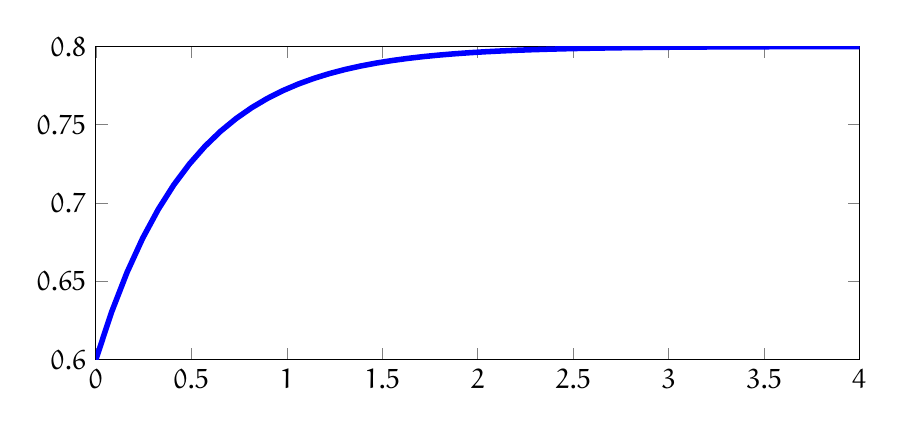
\begin{tikzpicture}

\begin{axis}[%
width=0.8\columnwidth,
height=1.566in,
at={(0.758in,0.481in)},
scale only axis,
xmin=0,
xmax=4,
ymin=0.6,
ymax=0.8,
axis background/.style={fill=white}
]
\addplot [color=blue, line width=2.0pt, forget plot]
  table[row sep=crcr]{%
0	0.6\\
0.0816326530612245	0.630126836686338\\
0.163265306122449	0.655715541929049\\
0.244897959183673	0.67744971345245\\
0.326530612244898	0.69590997579586\\
0.408163265306122	0.711589491595235\\
0.489795918367347	0.724907136335567\\
0.571428571428571	0.736218688535206\\
0.653061224489796	0.745826334305907\\
0.73469387755102	0.753986740201238\\
0.816326530612245	0.760917910018055\\
0.897959183673469	0.766805008729289\\
0.979591836734694	0.771805309133374\\
1.06122448979592	0.776052393369177\\
1.14285714285714	0.779659721539155\\
1.22448979591837	0.782723662775877\\
1.30612244897959	0.785326069726323\\
1.38775510204082	0.787536465230832\\
1.46938775510204	0.789413899613458\\
1.55102040816327	0.791008528200911\\
1.63265306122449	0.792362951213216\\
1.71428571428571	0.793513351821041\\
1.79591836734694	0.794490462772687\\
1.87755102040816	0.79532038741401\\
1.95918367346939	0.796025297034677\\
2.04081632653061	0.796624023170242\\
2.12244897959184	0.797132560683277\\
2.20408163265306	0.797564495063291\\
2.28571428571429	0.797931365360676\\
2.36734693877551	0.798242972450389\\
2.44897959183673	0.798507640860592\\
2.53061224489796	0.798732441160944\\
2.61224489795918	0.798923378851616\\
2.69387755102041	0.799085554799168\\
2.77551020408163	0.799223301505289\\
2.85714285714286	0.799340298848812\\
2.93877551020408	0.79943967239303\\
3.02040816326531	0.799524076884561\\
3.10204081632653	0.799595767174431\\
3.18367346938776	0.799656658456027\\
3.26530612244898	0.799708377429141\\
3.3469387755102	0.799752305756973\\
3.42857142857143	0.799789616977012\\
3.51020408163265	0.799821307851888\\
3.59183673469388	0.799848224997704\\
3.6734693877551	0.79987108750124\\
3.75510204081633	0.799890506130225\\
3.83673469387755	0.79990699964989\\
3.91836734693878	0.799921008681687\\
4	0.79993290747442\\
};
\end{axis}
\end{tikzpicture}%

\end{onlyenv}
\begin{onlyenv}<2>
\centering
% This file was created by matlab2tikz.
%
%The latest updates can be retrieved from
%  http://www.mathworks.com/matlabcentral/fileexchange/22022-matlab2tikz-matlab2tikz
%where you can also make suggestions and rate matlab2tikz.
%
\definecolor{mycolor1}{rgb}{0.00000,0.44700,0.74100}%
\definecolor{mycolor2}{rgb}{0.85000,0.32500,0.09800}%
%
\begin{tikzpicture}

\begin{axis}[%
width=0.8\columnwidth,
height=1.566in,
at={(0.772in,0.481in)},
scale only axis,
unbounded coords=jump,
xmin=0,
xmax=4,
ymin=0,
ymax=8,
axis background/.style={fill=white},
legend style={legend cell align=left, align=left, draw=none, fill=none}
]
\addplot [color=mycolor1, line width=2.0pt]
  table[row sep=crcr]{%
0	nan\\
0.0816326530612245	1.68330036826363\\
0.163265306122449	1.47673329001169\\
0.244897959183673	1.36626266101202\\
0.326530612244898	1.2908014981932\\
0.408163265306122	1.23317663492977\\
0.489795918367347	1.18629607215855\\
0.571428571428571	1.14659303888878\\
0.653061224489796	1.11203685870951\\
0.73469387755102	1.08136671518844\\
0.816326530612245	1.05374749742461\\
0.897959183673469	1.02859747768048\\
0.979591836734694	1.00549468690936\\
1.06122448979592	0.984122686879926\\
1.14285714285714	0.964237493141336\\
1.22448979591837	0.945646515046001\\
1.30612244897959	0.928194651744788\\
1.38775510204082	0.911754822027989\\
1.46938775510204	0.896221336642468\\
1.55102040816327	0.881505147743549\\
1.63265306122449	0.867530370770968\\
1.71428571428571	0.854231689087503\\
1.79591836734694	0.841552383912326\\
1.87755102040816	0.829442815563119\\
1.95918367346939	0.817859236028562\\
2.04081632653061	0.806762848600086\\
2.12244897959184	0.79611905437003\\
2.20408163265306	0.78589684193437\\
2.28571428571429	0.77606828817652\\
2.36734693877551	0.766608146185343\\
2.44897959183673	0.757493502237032\\
2.53061224489796	0.748703488049281\\
2.61224489795918	0.740219037669766\\
2.69387755102041	0.73202268071176\\
2.77551020408163	0.724098365420861\\
2.85714285714286	0.716431306404549\\
2.93877551020408	0.709007852891674\\
3.02040816326531	0.70181537419126\\
3.10204081632653	0.694842159647115\\
3.18367346938776	0.688077330878636\\
3.26530612244898	0.681510764490178\\
3.3469387755102	0.675133023744686\\
3.42857142857143	0.668935297949357\\
3.51020408163265	0.662909348505296\\
3.59183673469388	0.657047460739418\\
3.6734693877551	0.651342400773193\\
3.75510204081633	0.645787376795119\\
3.83673469387755	0.640376004196829\\
3.91836734693878	0.635102274110182\\
4	0.629960524947436\\
};
\addlegendentry{$\Phi{}_\alpha\text{(s)}$}

\addplot [color=mycolor2, line width=2.0pt]
  table[row sep=crcr]{%
0	nan\\
0.0816326530612245	7.27737023703986\\
0.163265306122449	4.14766839850376\\
0.244897959183673	2.98868837585645\\
0.326530612244898	2.37255689917213\\
0.408163265306122	1.98673890714734\\
0.489795918367347	1.7210430975732\\
0.571428571428571	1.5262607923174\\
0.653061224489796	1.37697773954811\\
0.73469387755102	1.25869521596466\\
0.816326530612245	1.16251758888532\\
0.897959183673469	1.08267460090185\\
0.979591836734694	1.01525482593162\\
1.06122448979592	0.957510384498091\\
1.14285714285714	0.907452786501162\\
1.22448979591837	0.863606700466653\\
1.30612244897959	0.824853923216218\\
1.38775510204082	0.79033114811648\\
1.46938775510204	0.759361028052662\\
1.55102040816327	0.731404511653325\\
1.63265306122449	0.70602715551696\\
1.71428571428571	0.682874846233408\\
1.79591836734694	0.661655997253038\\
1.87755102040816	0.642128288603692\\
1.95918367346939	0.624088650199998\\
2.04081632653061	0.607365598019616\\
2.12244897959184	0.591813301751295\\
2.20408163265306	0.577306943474895\\
2.28571428571429	0.563739050629123\\
2.36734693877551	0.55101657242411\\
2.44897959183673	0.539058529383344\\
2.53061224489796	0.527794108923091\\
2.61224489795918	0.517161111128817\\
2.69387755102041	0.507104671744848\\
2.77551020408163	0.497576206290217\\
2.85714285714286	0.488532531829876\\
2.93877551020408	0.479935132438889\\
3.02040816326531	0.471749541626391\\
3.10204081632653	0.463944820527803\\
3.18367346938776	0.456493114954787\\
3.26530612244898	0.449369277723879\\
3.3469387755102	0.442550545295008\\
3.42857142857143	0.436016259809851\\
3.51020408163265	0.42974762925365\\
3.59183673469388	0.423727519768175\\
3.6734693877551	0.417940275190244\\
3.75510204081633	0.41237155973486\\
3.83673469387755	0.407008220427056\\
3.91836734693878	0.401838166444761\\
4	0.39685026299205\\
};
\addlegendentry{$\Psi{}_\alpha\text{(s)}$}

\end{axis}
\end{tikzpicture}%

\end{onlyenv}
\end{column}
\end{columns}

\end{frame}

\begin{frame}[fragile]{An example: inverting the Laplace transform}

\begin{columns}
\begin{column}{0.65\columnwidth}
We can then solve 
\[
\begin{cases}
{}_{S}D^{\alpha(t)}_{[0,t]} y(t) = -0.5 y(t), \\
y(0) = 1
\end{cases}
\]
\begin{onlyenv}<1>
by first setting the various quantities:
\definecolor{bg}{rgb}{0.95,0.95,0.95}
\begin{minted}[bgcolor=bg,fontsize=\small,breaklines]{matlab}
y0 = 1;
lambda = 0.5;
Psi = @(s) s.^(-s.*A(s));
F = @(s) y0./(s.*(1 + lambda*Psi(s)));
\end{minted}
\end{onlyenv}
\begin{onlyenv}<2>
Then inverting the Laplace transform on a \textbf{parabolic contour}\vspace{-0.5em}
\definecolor{bg}{rgb}{0.95,0.95,0.95}
\begin{minted}[bgcolor=bg,fontsize=\small,breaklines]{matlab}
L = -log(eps); N = ceil(4*L/3/pi);
h = 2*pi/L + L/2/pi/N^2; p = L^3/4/pi^2/N^2;
u = (0:N)*h; f = zeros(size(t));
for n = 1:length(t)
 mu = p/t(n);
 z = mu*(u*1i + 1).^2; z1 = 2*mu*(1i-u);
 G = exp(z.*t(n)).*F(z).*z1;
 f(n) = (imag(G(1))/2+sum(imag(G(2:N+1))))*h/pi;
end
\end{minted}
\end{onlyenv}
\begin{onlyenv}<3>
And we can comapre the solution with the one obtained for the two fixed orders, observing
that indeed we transition from one behavior to the other:
\definecolor{bg}{rgb}{0.95,0.95,0.95}
\begin{minted}[bgcolor=bg,fontsize=\footnotesize,breaklines]{matlab}
f_fun = @(t,y) -lambda*y; 
J_fun = @(t,y) -lambda;
t0 = 0; T = 4; h = 1e-2;
alpha = alpha1;
[t1, y1] = fde_pi2_im(alpha,f_fun,J_fun,t0,T,y0,h);
alpha = alpha2;
[t2, y2] = fde_pi2_im(alpha,f_fun,J_fun,t0,T,y0,h);
\end{minted}
\end{onlyenv}
\end{column}
\begin{column}{0.35\columnwidth}
\begin{onlyenv}<2>
\centering

% This file was created by matlab2tikz.
%
%The latest updates can be retrieved from
%  http://www.mathworks.com/matlabcentral/fileexchange/22022-matlab2tikz-matlab2tikz
%where you can also make suggestions and rate matlab2tikz.
%
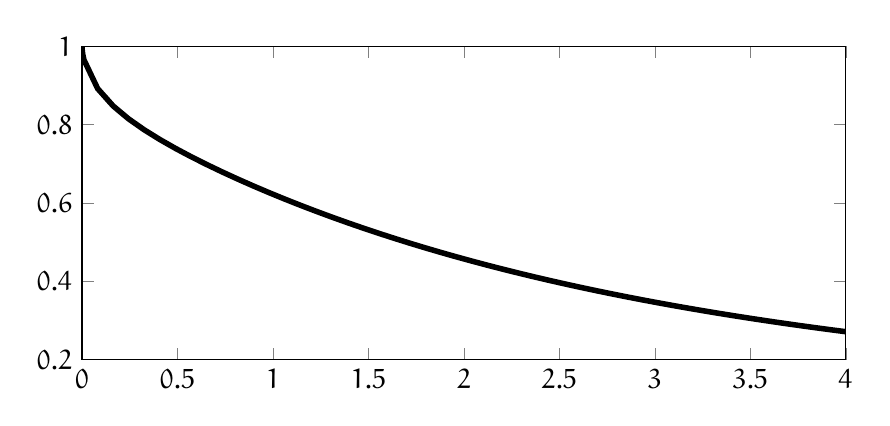
\begin{tikzpicture}

\begin{axis}[%
width=0.8\columnwidth,
height=1.566in,
at={(0.772in,0.481in)},
scale only axis,
xmin=0,
xmax=4,
ymin=0.2,
ymax=1,
axis background/.style={fill=white}
]
\addplot [color=black, line width=2.0pt, forget plot]
  table[row sep=crcr]{%
1e-06	0.99985945281503\\
1.62377673918872e-06	0.999812015468347\\
2.63665089873036e-06	0.999748570328325\\
4.2813323987194e-06	0.999663718165724\\
6.95192796177561e-06	0.999550240818276\\
1.12883789168469e-05	0.999398490214841\\
1.83298071083244e-05	0.999195573693794\\
2.97635144163132e-05	0.998924268999658\\
4.83293023857175e-05	0.998561581690418\\
7.84759970351461e-05	0.998076831644889\\
0.000127427498570313	0.997429123460756\\
0.000206913808111479	0.996564018311265\\
0.000335981828628378	0.99540918507009\\
0.000545559478116852	0.993868773648555\\
0.000885866790410082	0.991816239797825\\
0.00143844988828766	0.989085390230968\\
0.00233572146909012	0.985459568020997\\
0.00379269019073225	0.9806592565752\\
0.00615848211066026	0.974329080912414\\
0.01	0.966026356177728\\
0.0816326530612245	0.892565483796608\\
0.163265306122449	0.847898945376946\\
0.244897959183673	0.814669232599745\\
0.326530612244898	0.786846586681218\\
0.408163265306122	0.762165673171535\\
0.489795918367347	0.739546549619429\\
0.571428571428571	0.718407405352986\\
0.653061224489796	0.698409485556817\\
0.73469387755102	0.679344022686494\\
0.816326530612245	0.661076181349377\\
0.897959183673469	0.64351505819631\\
0.979591836734694	0.6265967187868\\
1.06122448979592	0.610274206995167\\
1.14285714285714	0.594511476844926\\
1.22448979591837	0.579279619119272\\
1.30612244897959	0.564554472535036\\
1.38775510204082	0.5503150909516\\
1.46938775510204	0.536542750180628\\
1.55102040816327	0.523220300136689\\
1.63265306122449	0.510331740590373\\
1.71428571428571	0.497861942933147\\
1.79591836734694	0.485796467816106\\
1.87755102040816	0.474121445906267\\
1.95918367346939	0.462823500176659\\
2.04081632653061	0.45188969542084\\
2.12244897959184	0.441307505468505\\
2.20408163265306	0.43106479175532\\
2.28571428571429	0.421149789022288\\
2.36734693877551	0.411551095345118\\
2.44897959183673	0.402257664653711\\
2.53061224489796	0.393258800549416\\
2.61224489795918	0.384544150663481\\
2.69387755102041	0.376103701093178\\
2.77551020408163	0.367927770647054\\
2.85714285714286	0.360007004759714\\
2.93877551020408	0.352332369020012\\
3.02040816326531	0.344895142309203\\
3.10204081632653	0.337686909577856\\
3.18367346938776	0.330699554308145\\
3.26530612244898	0.323925250717041\\
3.3469387755102	0.317356455758895\\
3.42857142857143	0.310985900984583\\
3.51020408163265	0.304806584311537\\
3.59183673469388	0.2988117617541\\
3.6734693877551	0.292994939158573\\
3.75510204081633	0.287349863982067\\
3.83673469387755	0.281870517148952\\
3.91836734693878	0.276551105013698\\
4	0.271386051454475\\
};
\end{axis}
\end{tikzpicture}%

\end{onlyenv}
\begin{onlyenv}<3>
\centering

% This file was created by matlab2tikz.
%
%The latest updates can be retrieved from
%  http://www.mathworks.com/matlabcentral/fileexchange/22022-matlab2tikz-matlab2tikz
%where you can also make suggestions and rate matlab2tikz.
%
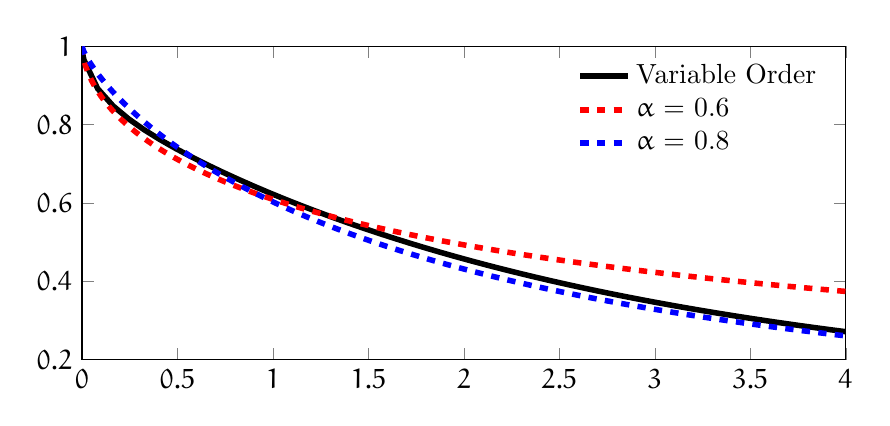
\begin{tikzpicture}

\begin{axis}[%
width=0.8\columnwidth,
height=1.566in,
at={(0.772in,0.481in)},
scale only axis,
xmin=0,
xmax=4,
ymin=0.2,
ymax=1,
axis background/.style={fill=white},
legend style={legend cell align=left, align=left, draw=none, fill=none}
]
\addplot [color=black, line width=2.0pt]
  table[row sep=crcr]{%
1e-06	0.99985945281503\\
1.62377673918872e-06	0.999812015468347\\
2.63665089873036e-06	0.999748570328325\\
4.2813323987194e-06	0.999663718165724\\
6.95192796177561e-06	0.999550240818276\\
1.12883789168469e-05	0.999398490214841\\
1.83298071083244e-05	0.999195573693794\\
2.97635144163132e-05	0.998924268999658\\
4.83293023857175e-05	0.998561581690418\\
7.84759970351461e-05	0.998076831644889\\
0.000127427498570313	0.997429123460756\\
0.000206913808111479	0.996564018311265\\
0.000335981828628378	0.99540918507009\\
0.000545559478116852	0.993868773648555\\
0.000885866790410082	0.991816239797825\\
0.00143844988828766	0.989085390230968\\
0.00233572146909012	0.985459568020997\\
0.00379269019073225	0.9806592565752\\
0.00615848211066026	0.974329080912414\\
0.01	0.966026356177728\\
0.0816326530612245	0.892565483796608\\
0.163265306122449	0.847898945376946\\
0.244897959183673	0.814669232599745\\
0.326530612244898	0.786846586681218\\
0.408163265306122	0.762165673171535\\
0.489795918367347	0.739546549619429\\
0.571428571428571	0.718407405352986\\
0.653061224489796	0.698409485556817\\
0.73469387755102	0.679344022686494\\
0.816326530612245	0.661076181349377\\
0.897959183673469	0.64351505819631\\
0.979591836734694	0.6265967187868\\
1.06122448979592	0.610274206995167\\
1.14285714285714	0.594511476844926\\
1.22448979591837	0.579279619119272\\
1.30612244897959	0.564554472535036\\
1.38775510204082	0.5503150909516\\
1.46938775510204	0.536542750180628\\
1.55102040816327	0.523220300136689\\
1.63265306122449	0.510331740590373\\
1.71428571428571	0.497861942933147\\
1.79591836734694	0.485796467816106\\
1.87755102040816	0.474121445906267\\
1.95918367346939	0.462823500176659\\
2.04081632653061	0.45188969542084\\
2.12244897959184	0.441307505468505\\
2.20408163265306	0.43106479175532\\
2.28571428571429	0.421149789022288\\
2.36734693877551	0.411551095345118\\
2.44897959183673	0.402257664653711\\
2.53061224489796	0.393258800549416\\
2.61224489795918	0.384544150663481\\
2.69387755102041	0.376103701093178\\
2.77551020408163	0.367927770647054\\
2.85714285714286	0.360007004759714\\
2.93877551020408	0.352332369020012\\
3.02040816326531	0.344895142309203\\
3.10204081632653	0.337686909577856\\
3.18367346938776	0.330699554308145\\
3.26530612244898	0.323925250717041\\
3.3469387755102	0.317356455758895\\
3.42857142857143	0.310985900984583\\
3.51020408163265	0.304806584311537\\
3.59183673469388	0.2988117617541\\
3.6734693877551	0.292994939158573\\
3.75510204081633	0.287349863982067\\
3.83673469387755	0.281870517148952\\
3.91836734693878	0.276551105013698\\
4	0.271386051454475\\
};
\addlegendentry{Variable Order}

\addplot [color=red, dashed, line width=2.0pt]
  table[row sep=crcr]{%
0	1\\
0.01	0.965454735760595\\
0.02	0.948408474951188\\
0.03	0.934916090364983\\
0.04	0.923369666616415\\
0.05	0.913112846256015\\
0.06	0.903797541691083\\
0.07	0.895211581644195\\
0.08	0.887213774644633\\
0.09	0.879704269300106\\
0.1	0.872609214523307\\
0.11	0.865872076245356\\
0.12	0.859448378788554\\
0.13	0.853302347355168\\
0.14	0.847404671067432\\
0.15	0.841730959358648\\
0.16	0.836260644993323\\
0.17	0.830976184707633\\
0.18	0.825862464005419\\
0.19	0.820906345550645\\
0.2	0.81609632079743\\
0.21	0.811422237288974\\
0.22	0.806875082378292\\
0.23	0.802446809669881\\
0.24	0.798130198258212\\
0.25	0.793918737460867\\
0.26	0.789806531596382\\
0.27	0.785788220686235\\
0.28	0.781858913928369\\
0.29	0.778014133503859\\
0.3	0.774249766811693\\
0.31	0.770562025629556\\
0.32	0.76694741100587\\
0.33	0.763402682925332\\
0.34	0.759924833974275\\
0.35	0.756511066376659\\
0.36	0.753158771885543\\
0.37	0.749865514105732\\
0.38	0.746629012896073\\
0.39	0.743447130558619\\
0.4	0.74031785956948\\
0.41	0.737239311645176\\
0.42	0.734209707970151\\
0.43	0.73122737043752\\
0.44	0.72829071377693\\
0.45	0.725398238461648\\
0.46	0.722548524302168\\
0.47	0.719740224646481\\
0.48	0.7169720611179\\
0.49	0.714242818830479\\
0.5	0.711551342029887\\
0.51	0.708896530114122\\
0.52	0.706277333994267\\
0.53	0.70369275276019\\
0.54	0.701141830620453\\
0.55	0.698623654089201\\
0.56	0.696137349395998\\
0.57	0.693682080097272\\
0.58	0.691257044870472\\
0.59	0.688861475473999\\
0.6	0.686494634857926\\
0.61	0.684155815412006\\
0.62	0.681844337338937\\
0.63	0.679559547142035\\
0.64	0.677300816217631\\
0.65	0.675067539543367\\
0.66	0.672859134454544\\
0.67	0.670675039501335\\
0.68	0.668514713380436\\
0.69	0.666377633935223\\
0.7	0.664263297219181\\
0.71	0.662171216617691\\
0.72	0.660100922023812\\
0.73	0.658051959064017\\
0.74	0.656023888370228\\
0.75	0.654016284894789\\
0.76	0.652028737265324\\
0.77	0.650060847176635\\
0.78	0.648112228817095\\
0.79	0.646182508327173\\
0.8	0.644271323287839\\
0.81	0.642378322236949\\
0.82	0.640503164211678\\
0.83	0.638645518315349\\
0.84	0.636805063307016\\
0.85	0.634981487212478\\
0.86	0.633174486955178\\
0.87	0.631383768005952\\
0.88	0.629609044050316\\
0.89	0.627850036672282\\
0.9	0.62610647505374\\
0.91	0.624378095688385\\
0.92	0.622664642109425\\
0.93	0.620965864630209\\
0.94	0.619281520097079\\
0.95	0.617611371653663\\
0.96	0.615955188516082\\
0.97	0.614312745758357\\
0.98	0.612683824107499\\
0.99	0.61106820974776\\
1	0.609465694133521\\
1.01	0.607876073810368\\
1.02	0.606299150243912\\
1.03	0.60473472965598\\
1.04	0.603182622867757\\
1.05	0.601642645149466\\
1.06	0.600114616076447\\
1.07	0.598598359391041\\
1.08	0.597093702870207\\
1.09	0.595600478198503\\
1.1	0.594118520846112\\
1.11	0.592647669951821\\
1.12	0.591187768210495\\
1.13	0.589738661765074\\
1.14	0.588300200102675\\
1.15	0.58687223595472\\
1.16	0.585454625200841\\
1.17	0.584047226776482\\
1.18	0.582649902583866\\
1.19	0.581262517406349\\
1.2	0.579884938825919\\
1.21	0.5785170371436\\
1.22	0.577158685302954\\
1.23	0.575809758816118\\
1.24	0.574470135692615\\
1.25	0.573139696370589\\
1.26	0.571818323650541\\
1.27	0.570505902631318\\
1.28	0.569202320648323\\
1.29	0.567907467213863\\
1.3	0.566621233959445\\
1.31	0.565343514580191\\
1.32	0.564074204780914\\
1.33	0.562813202224129\\
1.34	0.56156040647972\\
1.35	0.560315718976281\\
1.36	0.559079042953976\\
1.37	0.557850283419065\\
1.38	0.556629347099709\\
1.39	0.555416142403313\\
1.4	0.554210579375151\\
1.41	0.553012569658348\\
1.42	0.551822026455002\\
1.43	0.550638864488657\\
1.44	0.549462999967812\\
1.45	0.548294350550572\\
1.46	0.547132835310399\\
1.47	0.545978374702871\\
1.48	0.544830890533459\\
1.49	0.543690305926219\\
1.5	0.542556545293441\\
1.51	0.541429534306176\\
1.52	0.540309199865667\\
1.53	0.53919547007546\\
1.54	0.538088274214565\\
1.55	0.536987542711113\\
1.56	0.535893207116977\\
1.57	0.534805200082971\\
1.58	0.533723455334808\\
1.59	0.53264790764973\\
1.6	0.53157849283375\\
1.61	0.530515147699552\\
1.62	0.529457810044979\\
1.63	0.5284064186321\\
1.64	0.527360913166877\\
1.65	0.526321234279321\\
1.66	0.525287323504258\\
1.67	0.524259123262508\\
1.68	0.523236576842658\\
1.69	0.522219628383217\\
1.7	0.52120822285534\\
1.71	0.520202306045893\\
1.72	0.519201824541058\\
1.73	0.518206725710287\\
1.74	0.51721695769065\\
1.75	0.516232469371695\\
1.76	0.515253210380534\\
1.77	0.514279131067425\\
1.78	0.513310182491665\\
1.79	0.512346316407801\\
1.8	0.511387485252261\\
1.81	0.510433642130245\\
1.82	0.509484740802955\\
1.83	0.508540735675161\\
1.84	0.507601581783019\\
1.85	0.506667234782162\\
1.86	0.505737650936306\\
1.87	0.504812787105665\\
1.88	0.50389260073616\\
1.89	0.502977049848463\\
1.9	0.502066093027599\\
1.91	0.501159689412578\\
1.92	0.500257798686407\\
1.93	0.499360381066205\\
1.94	0.498467397293722\\
1.95	0.497578808625815\\
1.96	0.496694576825457\\
1.97	0.495814664152736\\
1.98	0.494939033355955\\
1.99	0.494067647663319\\
2	0.49320047077443\\
2.01	0.492337466852073\\
2.02	0.49147860051434\\
2.03	0.490623836826711\\
2.04	0.489773141294466\\
2.05	0.48892647985512\\
2.06	0.488083818871145\\
2.07	0.487245125122849\\
2.08	0.48641036580123\\
2.09	0.485579508501269\\
2.1	0.484752521215093\\
2.11	0.483929372325451\\
2.12	0.483110030599259\\
2.13	0.482294465181287\\
2.14	0.481482645587973\\
2.15	0.48067454170149\\
2.16	0.479870123763612\\
2.17	0.479069362370131\\
2.18	0.478272228465068\\
2.19	0.477478693335046\\
2.2	0.476688728603995\\
2.21	0.475902306227701\\
2.22	0.475119398488603\\
2.23	0.474339977990611\\
2.24	0.47356401765414\\
2.25	0.472791490711234\\
2.26	0.472022370700533\\
2.27	0.471256631462796\\
2.28	0.470494247136023\\
2.29	0.469735192151035\\
2.3	0.468979441227016\\
2.31	0.468226969367038\\
2.32	0.467477751853853\\
2.33	0.46673176424566\\
2.34	0.465988982371936\\
2.35	0.465249382329406\\
2.36	0.464512940478109\\
2.37	0.463779633437398\\
2.38	0.463049438082213\\
2.39	0.462322331539273\\
2.4	0.461598291183345\\
2.41	0.460877294633762\\
2.42	0.460159319750691\\
2.43	0.459444344631781\\
2.44	0.458732347608719\\
2.45	0.45802330724377\\
2.46	0.457317202326646\\
2.47	0.4566140118711\\
2.48	0.455913715111858\\
2.49	0.455216291501405\\
2.5	0.454521720707029\\
2.51	0.453829982607717\\
2.52	0.45314105729119\\
2.53	0.452454925051044\\
2.54	0.451771566383893\\
2.55	0.451090961986544\\
2.56	0.45041309275317\\
2.57	0.449737939772763\\
2.58	0.449065484326309\\
2.59	0.448395707884318\\
2.6	0.44772859210403\\
2.61	0.447064118827202\\
2.62	0.446402270077303\\
2.63	0.445743028057344\\
2.64	0.445086375147259\\
2.65	0.444432293901691\\
2.66	0.443780767047593\\
2.67	0.443131777482012\\
2.68	0.442485308269778\\
2.69	0.441841342641341\\
2.7	0.441199863990558\\
2.71	0.44056085587266\\
2.72	0.439924302001986\\
2.73	0.439290186250153\\
2.74	0.438658492643738\\
2.75	0.438029205362517\\
2.76	0.437402308737444\\
2.77	0.436777787248619\\
2.78	0.436155625523536\\
2.79	0.43553580833502\\
2.8	0.434918320599629\\
2.81	0.434303147375708\\
2.82	0.433690273861431\\
2.83	0.433079685393509\\
2.84	0.43247136744494\\
2.85	0.431865305623712\\
2.86	0.431261485670794\\
2.87	0.430659893458958\\
2.88	0.430060514990578\\
2.89	0.429463336396462\\
2.9	0.428868343934084\\
2.91	0.428275523986192\\
2.92	0.427684863059069\\
2.93	0.427096347781163\\
2.94	0.426509964901737\\
2.95	0.425925701289105\\
2.96	0.425343543929538\\
2.97	0.424763479925527\\
2.98	0.424185496494623\\
2.99	0.423609580968064\\
3	0.423035720789249\\
3.01	0.422463903512575\\
3.02	0.421894116802117\\
3.03	0.421326348430263\\
3.04	0.420760586276515\\
3.05	0.420196818326139\\
3.06	0.419635032669075\\
3.07	0.419075217498632\\
3.08	0.418517361110217\\
3.09	0.417961451900412\\
3.1	0.417407478365553\\
3.11	0.416855429100655\\
3.12	0.416305292798387\\
3.13	0.415757058247845\\
3.14	0.415210714333446\\
3.15	0.414666250033907\\
3.16	0.414123654421251\\
3.17	0.413582916659602\\
3.18	0.413044026004231\\
3.19	0.412506971800541\\
3.2	0.411971743482973\\
3.21	0.411438330574181\\
3.22	0.410906722683939\\
3.23	0.410376909508135\\
3.24	0.409848880827974\\
3.25	0.409322626508874\\
3.26	0.408798136499634\\
3.27	0.408275400831507\\
3.28	0.407754409617314\\
3.29	0.407235153050514\\
3.3	0.406717621404318\\
3.31	0.406201805030909\\
3.32	0.405687694360614\\
3.33	0.405175279900884\\
3.34	0.404664552235584\\
3.35	0.404155502024212\\
3.36	0.403648120001026\\
3.37	0.40314239697425\\
3.38	0.402638323825372\\
3.39	0.40213589150828\\
3.4	0.401635091048423\\
3.41	0.401135913542357\\
3.42	0.400638350156602\\
3.43	0.400142392127281\\
3.44	0.39964803075908\\
3.45	0.399155257424806\\
3.46	0.398664063564415\\
3.47	0.398174440684545\\
3.48	0.397686380357749\\
3.49	0.397199874221728\\
3.5	0.396714913978745\\
3.51	0.396231491395063\\
3.52	0.395749598300082\\
3.53	0.395269226585796\\
3.54	0.394790368206218\\
3.55	0.394313015176617\\
3.56	0.393837159573074\\
3.57	0.393362793531656\\
3.58	0.392889909248031\\
3.59	0.392418498976642\\
3.6	0.391948555030389\\
3.61	0.391480069779851\\
3.62	0.391013035652675\\
3.63	0.390547445133158\\
3.64	0.390083290761644\\
3.65	0.389620565133908\\
3.66	0.389159260900702\\
3.67	0.38869937076712\\
3.68	0.388240887492086\\
3.69	0.387783803887962\\
3.7	0.387328112819742\\
3.71	0.3868738072049\\
3.72	0.386420880012569\\
3.73	0.385969324263249\\
3.74	0.385519133028096\\
3.75	0.385070299428749\\
3.76	0.384622816636586\\
3.77	0.384176677872231\\
3.78	0.383731876405329\\
3.79	0.383288405553776\\
3.8	0.382846258683606\\
3.81	0.38240542920815\\
3.82	0.381965910587891\\
3.83	0.381527696329848\\
3.84	0.381090779987161\\
3.85	0.380655155158831\\
3.86	0.380220815489028\\
3.87	0.379787754666793\\
3.88	0.379355966425708\\
3.89	0.378925444543274\\
3.9	0.37849618284074\\
3.91	0.378068175182414\\
3.92	0.377641415475635\\
3.93	0.377215897670018\\
3.94	0.376791615757224\\
3.95	0.376368563770678\\
3.96	0.375946735784948\\
3.97	0.375526125915546\\
3.98	0.375106728318539\\
3.99	0.374688537190103\\
4	0.37427154676624\\
};
\addlegendentry{$\alpha\text{ = 0.6}$}

\addplot [color=blue, dashed, line width=2.0pt]
  table[row sep=crcr]{%
0	1\\
0.01	0.986615567958287\\
0.02	0.97684386484309\\
0.03	0.968147919238833\\
0.04	0.960109347945969\\
0.05	0.952542557681489\\
0.06	0.945342947547023\\
0.07	0.938443581580288\\
0.08	0.931798048570864\\
0.09	0.925372326830631\\
0.1	0.919140433068334\\
0.11	0.913081887941111\\
0.12	0.907180141703392\\
0.13	0.901421545709484\\
0.14	0.89579465266347\\
0.15	0.890289724331427\\
0.16	0.884898375343351\\
0.17	0.879613309226363\\
0.18	0.874428118712843\\
0.19	0.869337131934843\\
0.2	0.864335292075015\\
0.21	0.859418061869075\\
0.22	0.854581346875462\\
0.23	0.849821433128472\\
0.24	0.845134935962682\\
0.25	0.840518757618899\\
0.26	0.835970051829036\\
0.27	0.831486194003016\\
0.28	0.827064755953894\\
0.29	0.822703484330496\\
0.3	0.81840028210262\\
0.31	0.814153192577749\\
0.32	0.80996038553125\\
0.33	0.805820145112144\\
0.34	0.80173085924923\\
0.35	0.79769101033197\\
0.36	0.793699166980012\\
0.37	0.789753976746848\\
0.38	0.785854159628703\\
0.39	0.781998502270503\\
0.4	0.778185852777691\\
0.41	0.774415116056677\\
0.42	0.770685249618164\\
0.43	0.766995259787192\\
0.44	0.763344198271724\\
0.45	0.75973115904825\\
0.46	0.756155275528597\\
0.47	0.752615717976791\\
0.48	0.749111691148932\\
0.49	0.745642432132472\\
0.5	0.74220720836419\\
0.51	0.738805315808724\\
0.52	0.735436077281649\\
0.53	0.73209884090304\\
0.54	0.728792978668962\\
0.55	0.725517885129851\\
0.56	0.722272976165931\\
0.57	0.719057687850861\\
0.58	0.715871475395797\\
0.59	0.712713812166815\\
0.6	0.709584188769442\\
0.61	0.706482112194582\\
0.62	0.703407105020797\\
0.63	0.70035870466832\\
0.64	0.697336462700633\\
0.65	0.694339944169905\\
0.66	0.691368727002819\\
0.67	0.688422401423752\\
0.68	0.685500569412466\\
0.69	0.682602844193743\\
0.7	0.679728849756657\\
0.71	0.676878220401321\\
0.72	0.674050600311185\\
0.73	0.671245643149046\\
0.74	0.668463011675234\\
0.75	0.665702377386323\\
0.76	0.662963420173125\\
0.77	0.660245827996639\\
0.78	0.657549296580712\\
0.79	0.654873529120479\\
0.8	0.652218236005452\\
0.81	0.6495831345564\\
0.82	0.646967948775149\\
0.83	0.644372409106524\\
0.84	0.641796252211652\\
0.85	0.639239220752055\\
0.86	0.636701063183739\\
0.87	0.634181533560838\\
0.88	0.631680391348212\\
0.89	0.629197401242434\\
0.9	0.626732333000812\\
0.91	0.62428496127788\\
0.92	0.621855065469017\\
0.93	0.619442429560792\\
0.94	0.617046841987681\\
0.95	0.614668095494777\\
0.96	0.612305987006232\\
0.97	0.609960317499105\\
0.98	0.60763089188233\\
0.99	0.605317518880571\\
1	0.603020010922687\\
1.01	0.600738184034588\\
1.02	0.598471857736286\\
1.03	0.59622085494293\\
1.04	0.593985001869529\\
1.05	0.591764127939459\\
1.06	0.589558065696176\\
1.07	0.587366650718371\\
1.08	0.585189721538175\\
1.09	0.583027119562313\\
1.1	0.580878688996143\\
1.11	0.578744276770368\\
1.12	0.576623732470387\\
1.13	0.574516908268016\\
1.14	0.572423658855696\\
1.15	0.570343841382896\\
1.16	0.568277315394656\\
1.17	0.566223942772283\\
1.18	0.564183587675938\\
1.19	0.562156116489201\\
1.2	0.560141397765397\\
1.21	0.558139302175707\\
1.22	0.55614970245895\\
1.23	0.554172473372929\\
1.24	0.55220749164739\\
1.25	0.550254635938395\\
1.26	0.548313786784159\\
1.27	0.546384826562234\\
1.28	0.544467639447997\\
1.29	0.542562111374441\\
1.3	0.540668129993129\\
1.31	0.538785584636351\\
1.32	0.53691436628037\\
1.33	0.535054367509817\\
1.34	0.533205482483016\\
1.35	0.531367606898458\\
1.36	0.529540637962094\\
1.37	0.527724474355668\\
1.38	0.525919016205886\\
1.39	0.524124165054481\\
1.4	0.522339823829109\\
1.41	0.520565896815056\\
1.42	0.518802289627666\\
1.43	0.517048909185654\\
1.44	0.51530566368496\\
1.45	0.513572462573461\\
1.46	0.511849216526311\\
1.47	0.510135837421874\\
1.48	0.508432238318363\\
1.49	0.50673833343107\\
1.5	0.505054038110181\\
1.51	0.50337926881916\\
1.52	0.501713943113681\\
1.53	0.500057979621152\\
1.54	0.498411298020583\\
1.55	0.496773819023248\\
1.56	0.495145464353562\\
1.57	0.493526156730529\\
1.58	0.491915819849691\\
1.59	0.490314378365469\\
1.6	0.488721757873909\\
1.61	0.487137884895913\\
1.62	0.485562686860782\\
1.63	0.483996092090259\\
1.64	0.48243802978285\\
1.65	0.480888429998558\\
1.66	0.479347223643956\\
1.67	0.477814342457672\\
1.68	0.4762897189961\\
1.69	0.474773286619493\\
1.7	0.473264979478425\\
1.71	0.471764732500416\\
1.72	0.470272481377064\\
1.73	0.46878816255125\\
1.74	0.467311713204738\\
1.75	0.465843071246119\\
1.76	0.464382175298829\\
1.77	0.462928964689588\\
1.78	0.461483379437088\\
1.79	0.460045360240726\\
1.8	0.458614848469906\\
1.81	0.45719178615327\\
1.82	0.455776115968311\\
1.83	0.454367781231184\\
1.84	0.452966725886712\\
1.85	0.451572894498585\\
1.86	0.450186232239815\\
1.87	0.44880668488335\\
1.88	0.447434198792862\\
1.89	0.446068720913776\\
1.9	0.444710198764432\\
1.91	0.443358580427455\\
1.92	0.44201381454127\\
1.93	0.44067585029186\\
1.94	0.439344637404551\\
1.95	0.438020126136108\\
1.96	0.436702267266879\\
1.97	0.435391012093154\\
1.98	0.43408631241962\\
1.99	0.432788120552047\\
2	0.431496389289961\\
2.01	0.430211071919713\\
2.02	0.428932122207348\\
2.03	0.427659494391917\\
2.04	0.426393143178665\\
2.05	0.425133023732604\\
2.06	0.42387909167192\\
2.07	0.422631303061767\\
2.08	0.421389614407983\\
2.09	0.420153982651014\\
2.1	0.418924365159929\\
2.11	0.417700719726568\\
2.12	0.41648300455969\\
2.13	0.415271178279448\\
2.14	0.414065199911725\\
2.15	0.412865028882668\\
2.16	0.411670625013325\\
2.17	0.410481948514479\\
2.18	0.409298959981303\\
2.19	0.408121620388376\\
2.2	0.406949891084667\\
2.21	0.405783733788603\\
2.22	0.404623110583206\\
2.23	0.403467983911521\\
2.24	0.402318316571671\\
2.25	0.401174071712529\\
2.26	0.400035212829069\\
2.27	0.398901703757974\\
2.28	0.39777350867329\\
2.29	0.396650592082112\\
2.3	0.395532918820416\\
2.31	0.394420454048926\\
2.32	0.393313163248954\\
2.33	0.392211012218463\\
2.34	0.391113967068109\\
2.35	0.390021994217396\\
2.36	0.388935060390819\\
2.37	0.387853132614124\\
2.38	0.386776178210667\\
2.39	0.385704164797665\\
2.4	0.38463706028274\\
2.41	0.383574832860328\\
2.42	0.382517451008267\\
2.43	0.38146488348436\\
2.44	0.380417099323118\\
2.45	0.379374067832149\\
2.46	0.378335758589405\\
2.47	0.377302141439507\\
2.48	0.376273186490898\\
2.49	0.375248864112611\\
2.5	0.374229144931224\\
2.51	0.373213999827941\\
2.52	0.372203399935523\\
2.53	0.371197316635411\\
2.54	0.370195721554865\\
2.55	0.369198586564112\\
2.56	0.368205883773664\\
2.57	0.367217585531367\\
2.58	0.366233664419858\\
2.59	0.365254093253871\\
2.6	0.364278845077642\\
2.61	0.363307893162116\\
2.62	0.36234121100279\\
2.63	0.361378772316789\\
2.64	0.360420551040638\\
2.65	0.359466521327824\\
2.66	0.358516657546219\\
2.67	0.357570934275894\\
2.68	0.35662932630668\\
2.69	0.355691808635924\\
2.7	0.354758356466141\\
2.71	0.353828945202875\\
2.72	0.352903550452458\\
2.73	0.351982148019772\\
2.74	0.351064713906165\\
2.75	0.350151224307369\\
2.76	0.349241655611347\\
2.77	0.348335984396257\\
2.78	0.347434187428454\\
2.79	0.346536241660468\\
2.8	0.345642124228987\\
2.81	0.34475181245303\\
2.82	0.343865283831901\\
2.83	0.342982516043356\\
2.84	0.342103486941742\\
2.85	0.34122817455616\\
2.86	0.340356557088604\\
2.87	0.339488612912192\\
2.88	0.338624320569444\\
2.89	0.337763658770447\\
2.9	0.336906606391184\\
2.91	0.336053142471858\\
2.92	0.335203246215151\\
2.93	0.334356896984663\\
2.94	0.333514074303151\\
2.95	0.332674757850996\\
2.96	0.331838927464652\\
2.97	0.331006563134986\\
2.98	0.330177645005757\\
2.99	0.329352153372136\\
3	0.328530068679141\\
3.01	0.327711371520102\\
3.02	0.326896042635356\\
3.03	0.326084062910536\\
3.04	0.325275413375449\\
3.05	0.32447007520241\\
3.06	0.323668029704836\\
3.07	0.322869258336141\\
3.08	0.322073742688047\\
3.09	0.32128146448941\\
3.1	0.320492405604884\\
3.11	0.319706548033559\\
3.12	0.318923873907643\\
3.13	0.318144365491264\\
3.14	0.317368005179123\\
3.15	0.316594775495316\\
3.16	0.315824659092012\\
3.17	0.315057638748352\\
3.18	0.314293697369101\\
3.19	0.31353281798356\\
3.2	0.312774983744361\\
3.21	0.312020177926259\\
3.22	0.311268383925133\\
3.23	0.310519585256577\\
3.24	0.309773765555174\\
3.25	0.309030908572921\\
3.26	0.308290998178512\\
3.27	0.3075540183561\\
3.28	0.306819953204189\\
3.29	0.306088786934699\\
3.3	0.305360503871876\\
3.31	0.304635088451156\\
3.32	0.303912525218294\\
3.33	0.303192798828244\\
3.34	0.302475894044303\\
3.35	0.301761795736888\\
3.36	0.301050488882803\\
3.37	0.300341958564296\\
3.38	0.299636189967688\\
3.39	0.298933168383035\\
3.4	0.298232879202827\\
3.41	0.297535307921003\\
3.42	0.296840440132368\\
3.43	0.29614826153135\\
3.44	0.295458757911423\\
3.45	0.294771915163981\\
3.46	0.29408771927756\\
3.47	0.293406156337043\\
3.48	0.292727212522783\\
3.49	0.292050874109546\\
3.5	0.291377127466134\\
3.51	0.290705959054118\\
3.52	0.290037355427253\\
3.53	0.289371303230656\\
3.54	0.288707789199901\\
3.55	0.288046800160428\\
3.56	0.287388323026583\\
3.57	0.286732344800938\\
3.58	0.286078852573553\\
3.59	0.28542783352108\\
3.6	0.284779274906259\\
3.61	0.284133164076974\\
3.62	0.283489488465537\\
3.63	0.282848235588188\\
3.64	0.282209393044061\\
3.65	0.281572948514749\\
3.66	0.280938889763432\\
3.67	0.280307204634348\\
3.68	0.279677881051986\\
3.69	0.279050907020281\\
3.7	0.27842627062237\\
3.71	0.277803960019513\\
3.72	0.277183963450536\\
3.73	0.276566269231464\\
3.74	0.275950865754424\\
3.75	0.2753377414874\\
3.76	0.274726884973407\\
3.77	0.274118284829771\\
3.78	0.273511929747958\\
3.79	0.272907808492423\\
3.8	0.272305909900342\\
3.81	0.271706222880846\\
3.82	0.271108736414646\\
3.83	0.270513439553228\\
3.84	0.269920321418372\\
3.85	0.26932937120156\\
3.86	0.268740578163515\\
3.87	0.268153931633289\\
3.88	0.267569421008338\\
3.89	0.2669870357533\\
3.9	0.266406765399913\\
3.91	0.265828599546177\\
3.92	0.265252527856162\\
3.93	0.264678540059133\\
3.94	0.264106625949197\\
3.95	0.263536775384808\\
3.96	0.2629689782881\\
3.97	0.262403224644663\\
3.98	0.261839504502778\\
3.99	0.261277807972978\\
4	0.260718125227619\\
};
\addlegendentry{$\alpha\text{ = 0.8}$}

\end{axis}
\end{tikzpicture}%

\end{onlyenv}
\end{column}
\end{columns}

\end{frame}

\begin{frame}{\faBinoculars\;Possible research directions}

\begin{itemize}
\item[\faBinoculars]<1-> Scarpi FDEs with more difficult dynamics, e.g., the vector case with a non-diagonalizable matrix, non-linear FDEs, \emph{etc.}
\item[\faBinoculars]<2-> Algorithms for the automatic selection of contours and parameters given the FDE.
\item[\faBinoculars]<3-> In the \emph{complex-network case} \cite{DIAZDIAZ2022111791} explored the case of standard time-fractional evolutions, what about \emph{distributed} or \emph{variable} order? Are they reasonable from a modeling point of view? Can we \textbf{efficiently} use them?
\item[\faBinoculars]<4-> All-at-once formulations for the \emph{other} FDEs?
\item[\faBinoculars]<5-> General poles for Rational Krylov methods for the computation of Mittag-Leffler matrix-function times vector algorithms?
\end{itemize}

\end{frame}

\section{Conclusions}

\begin{frame}{Conclusions}

In this \alert{\textbf{first part of the course}} we have dealt with
\begin{itemize}
\item[\faCog] Defining and analyzing properties of Riemann-Liouville integral and derivatives,
\item[\faCog] Defining and analyzing properties of Caputo integral and derivatives,
\item[\faCog] Existence, uniqueness and regularity of FDEs with Caputo derivatives,
\item[\faCog] Explored the connection between time-fractional derivatives and CTRW,
\item[\faCog] FDEs with mulitple, distributed and variable orders.
\end{itemize}
For what concerns \alert{\textbf{numerical methods}} we have seen
\begin{itemize}
\item[\faWrench] Product Integral Rules and Fractional Linear Multistep Methods for integrating FDEs,
\item[\faWrench] An overview of some inversion techniques for the Laplace Transform,
\item[\faWrench] Computation of the Mittag-Leffler function and its derivative on scalar and matrix arguments,
\item[\faWrench] Krylov methods for the computation of matrix functions.
\end{itemize}

\end{frame}

\begin{frame}{Programs for the (\emph{near}) future}

\only<1>{\centering 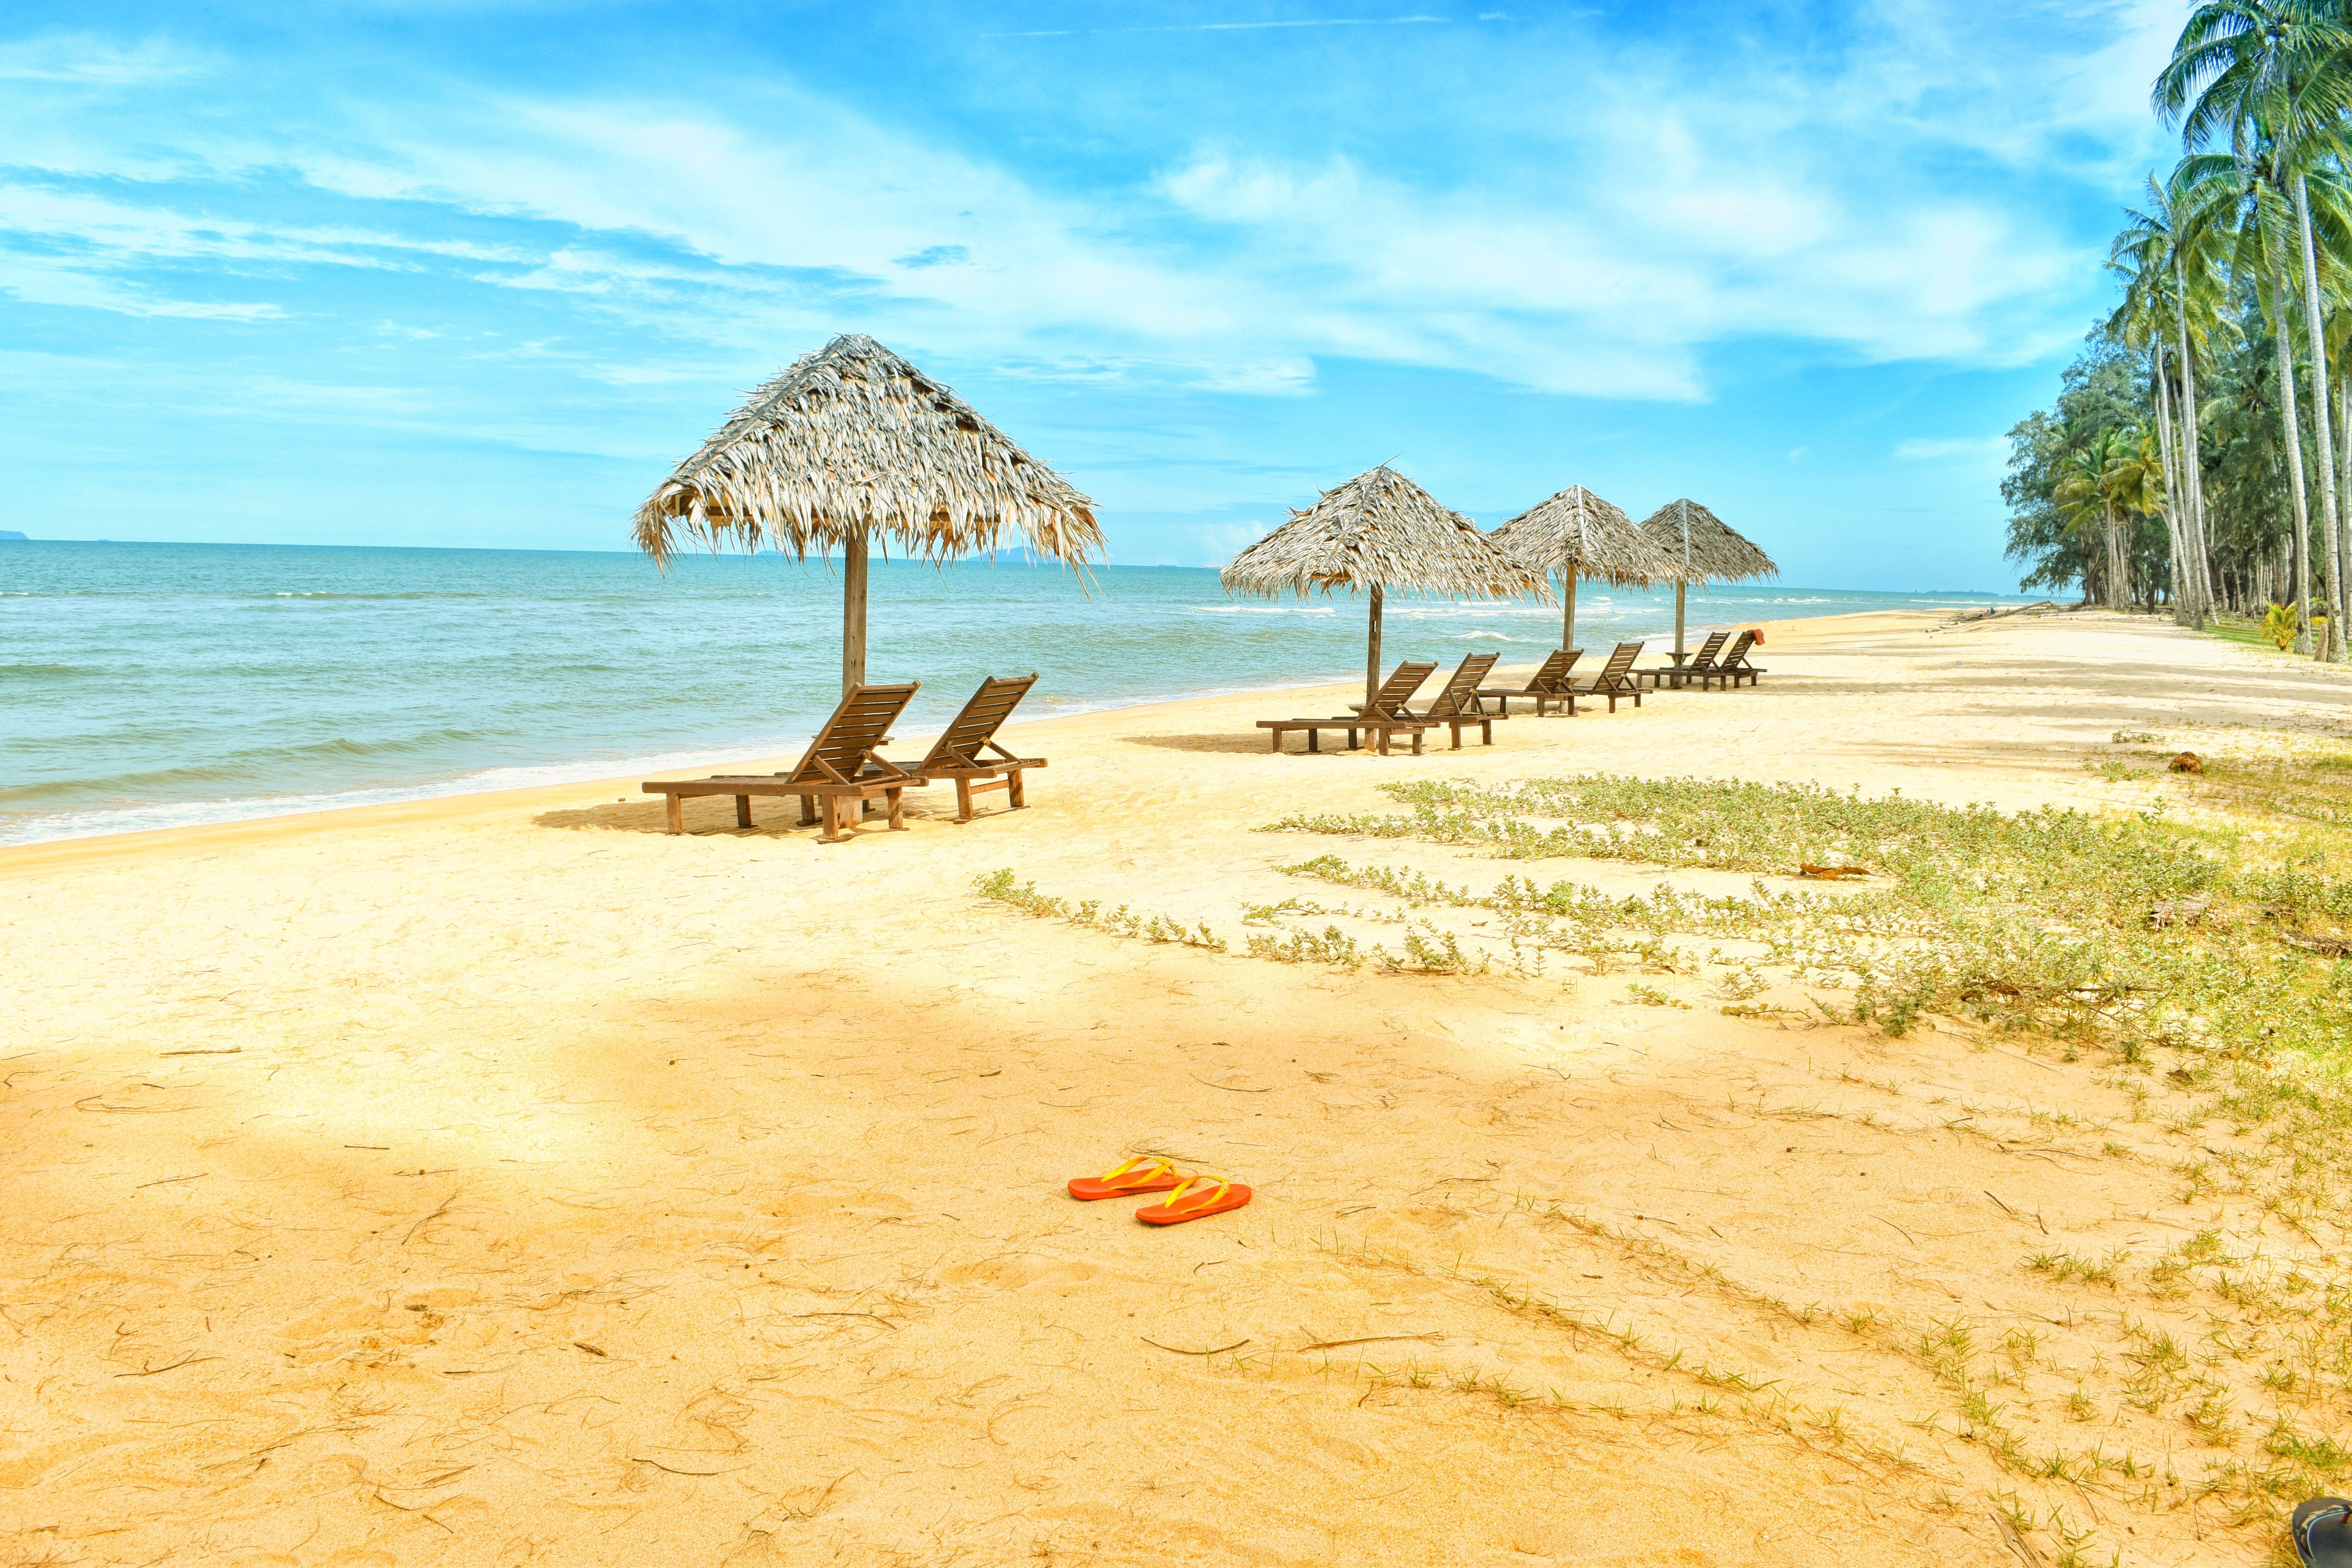
\includegraphics[width=0.75\columnwidth]{future.jpg}}

\end{frame}

%
%\begin{frame}{Extension to time dependent Networks}\vspace{1em}
%\begin{columns}
%\begin{column}{0.5\columnwidth}
%\centering
%
%\begin{animateinline}[controls,autoplay,loop]{50}
%	\multiframe{180}{rt=0+1}{%
%	\begin{tikzpicture}
%	\Vertex[x=1,y=0,color=orange]{A};
%	\Vertex[x=2,y=0,color=orange]{B};
%	\Vertex[x=3,y=0,color=orange]{C};
%	\Vertex[x=1,y=1,color=orange]{D};
%	\Vertex[x=2,y=1,color=orange]{E};
%	\Vertex[x=3,y=1,color=orange]{F};
%	\ifthenelse{\rt < 60}{%
%		\Edge(A)(B);
%		\Edge(B)(C);
%		\Edge(B)(E);
%	}{%
%		\ifthenelse{\rt < 120}{%
%			\Edge(A)(D);
%			\Edge(C)(F);
%		}{
%			\Edge(A)(F);
%			\Edge(C)(D);
%		}
%	}
%	\end{tikzpicture}
%	}
%\end{animateinline}
%\vspace{2em}
%
%Networks are often evolving over time, with edges appearing, disappearing, or changing their weight as time progresses.
%\end{column}
%\begin{column}{0.5\columnwidth}
%We consider time-dependent networks $G = (V,E(t))$ where
%\begin{itemize}
%	\item the nodes remain  unchanged,
%	\item the edge set $E(t)$ is time-dependent.
%\end{itemize}
%And represent it by $A(t) \, :\, \mathbb{R} \to \mathbb{R}^{n \times n}$ that can be (as function of $t$)
%\begin{itemize}
%	\item discontinuous and rapidly changing if we model instantaneous activities,
%	\item more regular for cases in which the edge weight varies between two values, e.g., $w_{i,j} \in [0,1]$.
%\end{itemize}
%\end{column}
%\end{columns}
%\end{frame}
%
%\begin{frame}{An idea of centrality based on dynamic communicability}
%We follow the idea introduced in [Grindrod, Higham 2014]:
%\begin{equation*}
%S(t + \Delta) = [ I + e^{-b \Delta} S(t) ] [I - \gamma A(t+\Delta) ]^{-\Delta} -I, \quad S(0) = 0, \quad   \gamma,b \in\mathbb{R}_{> 0}.
%\end{equation*}
%
%\textbf{\faLightbulb[regular]\,Idea:} matrix $S(t) \in \mathbb{R}^{n \times n}$ encodes in its $(i,j)$ entry the \alert{ability} of node $i$ \alert{to communicate} with node $j$ using edges {\it up to} time $t$ by \alert{counting the walks} that have appeared until time $t$. 
%
%\begin{itemize}
%	\item<2> For a discrete-time network sequence $\{t_i\}_{i=1}^{N}$ and $b=0$ 
%	\[ S(t_N) + I = \prod_{i=1}^{N} (I - \gamma A(t_i) )^{-1},\]
%	that is the \textbf{generalized Katz centrality measure} [Grindrod, et Al. 2011]
%	\item[\textcolor{red}{\faExclamationCircle}]<2> We need a restriction on $\gamma$ depending on $A(t)$
%\end{itemize}
%
%\end{frame}
%
%\begin{frame}{Dynamic communicability in the continuous limit}
%By letting $U(t) = I + S(t)$ (and after some Taylor expansions\ldots) one finds the \alert{continuous model}
%\begin{equation*}
%\begin{cases}
%U'(t) = - b (U(t)-I) - U(t) \log(I - \gamma A(t)), & t > 0,\\
%U(0) = I.
%\end{cases}
%\end{equation*}
%\begin{itemize}
%	\only<1-2>{\item[\textcolor{red}{\faExclamationCircle}] Existence of a principal determination of the matrix logarithm function is guaranteed when $ \gamma< \rho(A(t))^{-1}$ for all $t\geq 0$,
%	\item\,[Grindrod, Higham 2014] suggest replacing the resolvent function with an opportune matrix function $f(\gamma A(t))$}
%	\only<3>{
%	\item[{\faLightbulb[regular]}] To guarantee the existence of a principal determination of the matrix logarithm function in this case, we simply need $\gamma$ satisfying the requirements for well-posedness, \alert{no need to know the full temporal evolution}!
%	}
%	\item<2-3> As in the static case we employ Mittag--Leffler functions
%	\[f(\gamma A(t)) = E_\alpha(\gamma A(t)) \text{ for }\alpha\in (0,1],\] 
%	to again \textbf{interpolate between} the \textbf{resolvent} and the \textbf{exponential} behavior.
%\end{itemize}
%\end{frame}
%
%\begin{frame}{Dynamic broadcast/receive centralities}
%Let $A(t)$ be the adjacency matrix of a time-evolving network $G = (V,E(t))$. Suppose that $\alpha\in (0,1]$ and that $\gamma$ \alert{satisfies the well-posedness conditions}. Let $W(t)$ be the solution to  
%\[
%\begin{cases}
%W'(t) = - b(W(t)-I) - W(t) \log( E_{\alpha}(\gamma A(t)) ), & t > 0,\\
%W(0) = I.
%\end{cases}
%\]
%Then, for every node $i\in V$ we define its
%\begin{itemize}
%	\item[\faArrowAltCircleLeft] \textbf{dynamic broadcast centrality} as the $i$th entry of the vector: $\mathbf{b}(t)=W(t)\boldsymbol{1}$; and its
%	\item[\faArrowAltCircleRight] \textbf{dynamic receive centrality} as the $i$th entry of the vector $\mathbf{r}(t)=W^T(t)\bone$. 	
%\end{itemize}
%\end{frame}
%
%\begin{frame}[fragile]{Numerical Examples}
%
%\begin{columns}
%\begin{column}{0.6\columnwidth}
%\begin{animateinline}[controls,autoplay,loop]{50}
%	\multiframe{180}{rt=0+1}{%
%		\begin{tikzpicture}[scale=0.5]
%		\Vertices{phone.csv}
%		\ifthenelse{\rt < 90}{%
%			\Edges{phone1.csv}
%		}{%
%			\Edges{phone2.csv}
%		}
%		\end{tikzpicture}
%	}
%\end{animateinline}
%\end{column}
%\begin{column}{0.4\columnwidth}
%\small
%On a time interval $T = [0, 20]$, the adjacency matrix $A(t)$ switches between $A_1$ and $A_2$ on each each sub-interval $[i, i + 1)$
%\begin{equation*}
%A(t) = \begin{cases}
%A_1, & \operatorname{mod}(\lfloor t \rfloor,2) = 0 \\
%A_2, & \text{ otherwise},
%\end{cases}
%\end{equation*}
%Evaluate again the Kendall $\tau$ correlation between the \emph{broadcast} and \emph{receive} centrality measures obtained by the resolvent and ML model.
%\end{column}
%\end{columns}
%\end{frame}
%
%\begin{frame}{Numerical Examples}
%
%To compare them we fix for both the same value of $b=0.01$ and vary $\gamma \in (0,1]$
%\begin{columns}
%\begin{column}{0.5\columnwidth}
%\centering
%
%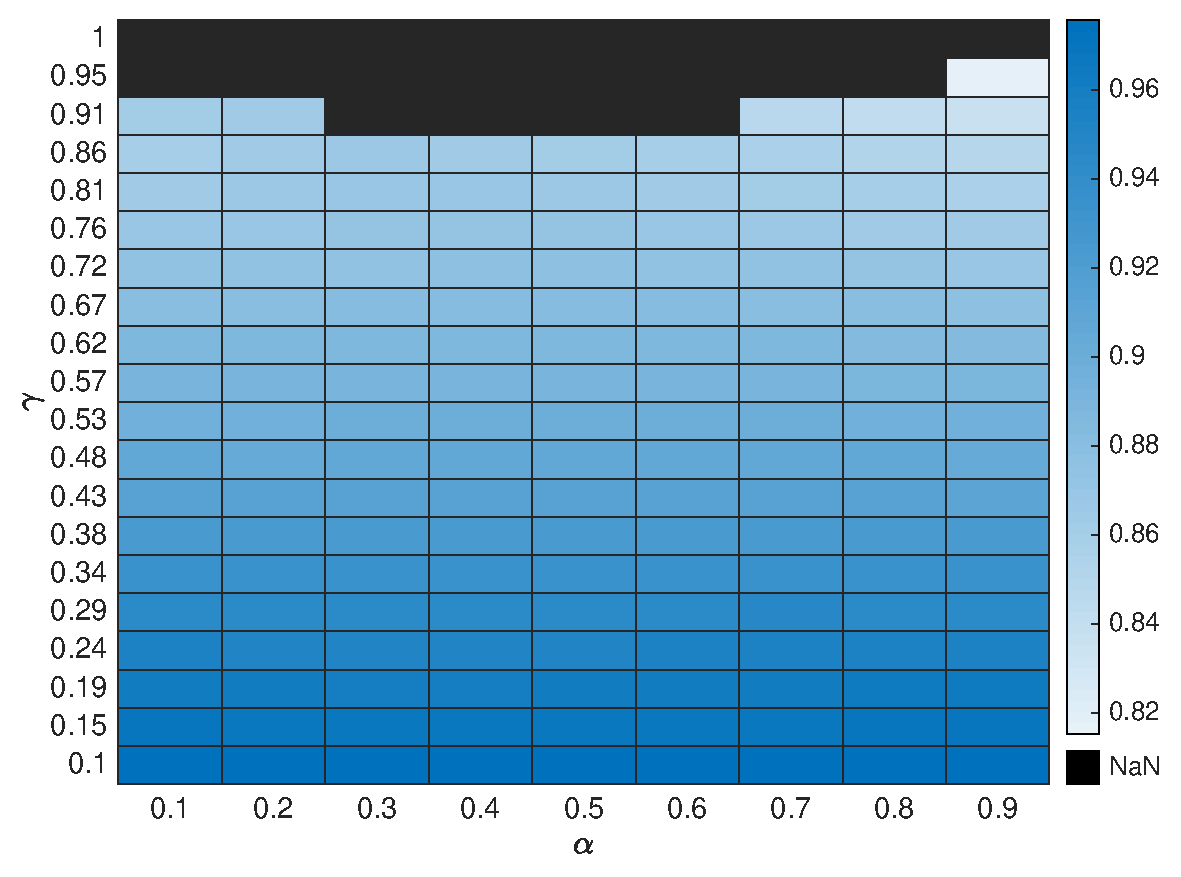
\includegraphics[width=0.8\columnwidth]{Figures/BroadcastCentrality.eps}
%
%Broadcast centrality
%
%\end{column}
%\begin{column}{0.5\columnwidth}
%\centering
%
%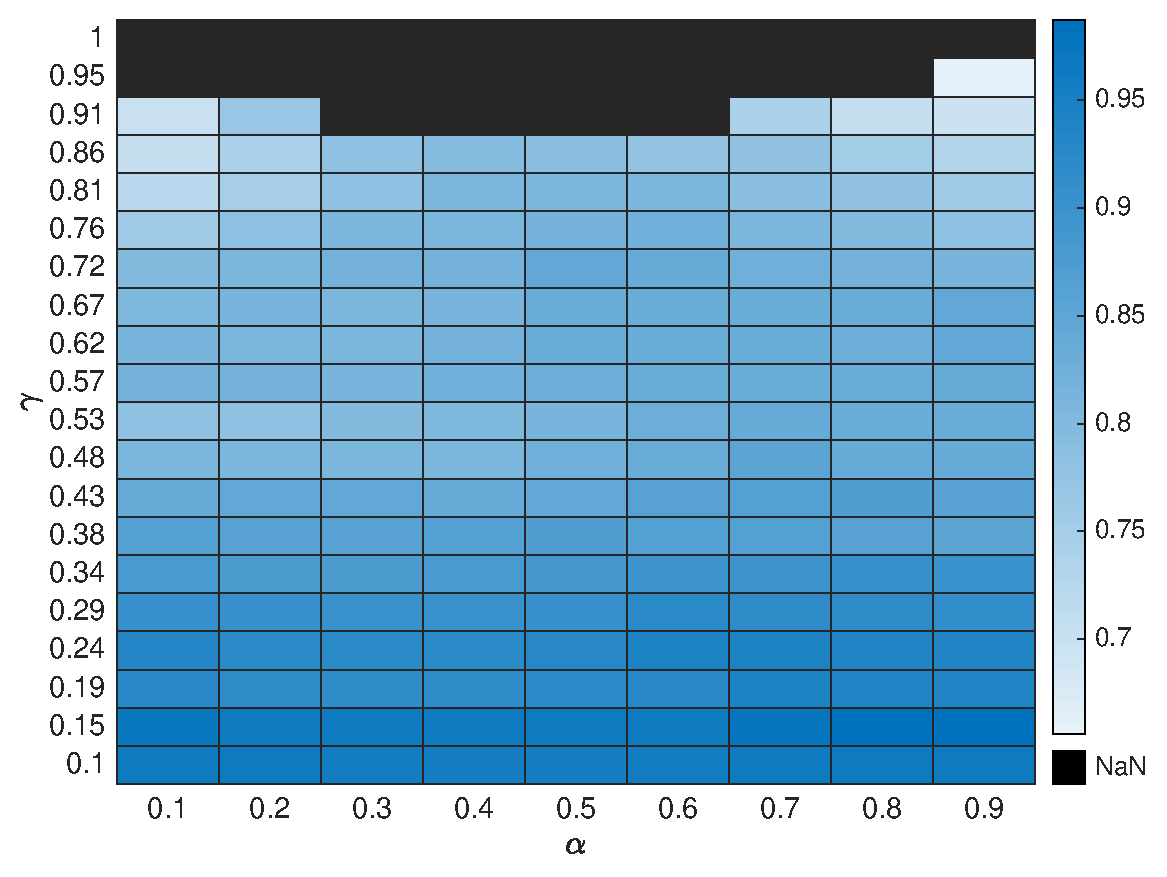
\includegraphics[width=0.8\columnwidth]{Figures/ReceiveCentrality.eps}
%
%Receive centrality
%
%\end{column}
%\end{columns}
%
%Measures are more sensitive to the variation of the scaling $\gamma$ than to the variation of $\alpha\to 1$.
%
%\end{frame}
%
%\begin{frame}{\faCompass\; The road goes ever on}
%
%\begin{itemize}
%	\item[\textcolor{Ao}{\faShoppingBasket}] We analyzed a general theory for ML-based centrality measures,
%	\item[\textcolor{Ao}{\faShoppingBasket}] Proved and numerically investigated asymptotics for the centrality measures,
%	\item[\textcolor{Ao}{\faShoppingBasket}] Described new ML-based centrality measures for time-evolving networks.
%\end{itemize}
%Plenty of things to explore
%\begin{itemize}
%	\item[\faWrench] Develop specialized techniques for the integration of the system of ODEs defining the dynamic centralities, compute $\log(E_\alpha(\gamma A(t)))\mathbf{v}$ in some clever way,
%	\item[\faSearch] Explore the connection with Caputo time-fractional derivatives,
%	\item[\faSearch] Is there any relation with networks of fractional oscillators/quantum fractional oscillators?
%\end{itemize}
%
%All the details are on
%\begin{itemize}
%\item[\faFile*] Francesca Arrigo, F. D., Mittag-Leffler functions and their applications in network science. \href{https://arxiv.org/abs/2103.12559}{arXiv:2103.12559}.
%\end{itemize}
%
%\end{frame}


\appendix

\section*{Bibliography}
{\unnumbered
	\begin{frame}[allowframebreaks,noframenumbering]{Bibliography}
	\small
	\printbibliography
	
\end{frame}
}

\end{document}